\documentclass[a4paper,twoside]{article}

\usepackage[a4paper]{geometry}
\usepackage{anysize}
%\marginsize{left}{right}{top}{bottom}
\marginsize{2.6cm}{2.6cm}{3.3cm}{4.2cm}

\usepackage{epsfig}
\usepackage{subfigure}
\usepackage{calc}
\usepackage{amssymb}
\usepackage{amstext}
\usepackage{amsmath}
\usepackage{amsthm}
\usepackage{multicol}
\usepackage{pslatex}
\usepackage{apalike}
\usepackage{SciTePress}
\usepackage[small]{caption}


\subfigtopskip=0pt
\subfigcapskip=0pt
\subfigbottomskip=0pt

%%%%%%%%%

\usepackage{url}
\usepackage{multirow}

\begin{document}

\title{\uppercase{3D Texture Synthesis for Modeling Realistic Organic Tissues}}

\author{\authorname{PRIETO Juan-Carlos\sup{1}, REVOL-MULLER Chantal\sup{1}, PEYRIN Fran\c coise\sup{1,2}, CAMELLITI Patrizia\sup{3} and ODET Christophe\sup{1}}
\affiliation{\sup{1} CREATIS, CNRS UMR 5220, Inserm U1044, Univ. de Lyon1, INSA-Lyon, 7 Avenue Jean Capelle 69621, Lyon, France}
\affiliation{\sup{2} ESRF, BP 220, 38043 Grenoble Cedex, France}
\affiliation{\sup{3} NHLI, Imperial College London, UK}
\email{\{prieto, chantal.muller, fran\c coise.peyrin, christophe.odet\}@creatis.insa-lyon.fr, p.camelliti@imperial.ac.uk}
}

\keywords{3D Texture Synthesis, Image-based Modeling, Organ Modeling, Histology, Patient-specific, Image/Mechanical Simulation, Virtual Human}


\abstract{
Virtual anatomy models show in detail characteristics of the 
human body systems. 
These models are based in surface representation of the structures
and lack information from the interior of the object. 
Creating models that represent the surface, the interior of the object and are able to
provide pathological information is the current challenge of research in life sciences. 
We present a method to synthesize realistic three-dimensional organic tissues starting from bidimensional textured multi-channel samples.
The method relies on an energy function that measures the 
difference between the reference texture and the synthesized object, through a distance metric
that compares perpendicular neighborhoods in the object to neighborhoods in the sample. When this
function is minimized by IRLS, the result is a solid object that resembles the sample at every slice.
In some cases, the optimization might be aided by adding the feature distance 
transform, calculated from a given binary mask. This allows to code large textured areas.
Multiple textures can also be provided to the optimization in order to create anistropic textures.
We apply our method starting from various micrometric images such as histology images or slices of Synchrotron Radiation Computed Micro-Tomography (SR$\mu$CT) images. 
A major advantage of our method is to extend 2D histological information to a 3D representation. 
We demonstrate the accuracy of the generated texture by comparing statistical and morphological parameters computed 
from the synthetic object with those obtained from the real object underlying the reference images. 
}

\onecolumn \maketitle \normalsize \vfill

\begin{figure*}
 \centering 
 \subfigure[]{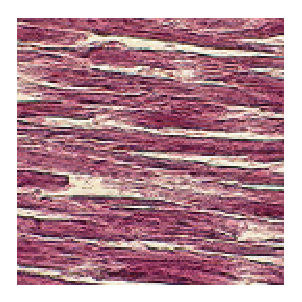
\epsfig{file = skeletal_muscle.eps, width = 1.6cm}}
 \subfigure[]{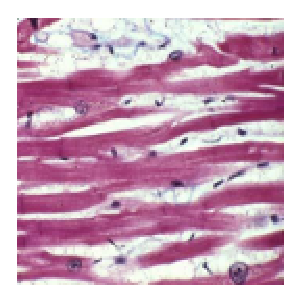
\epsfig{file = striescardiaques.eps, width = 1.6cm}}
 \subfigure[]{
\epsfig{file = myocyte.eps, width = 1.6cm}}
 \subfigure[]{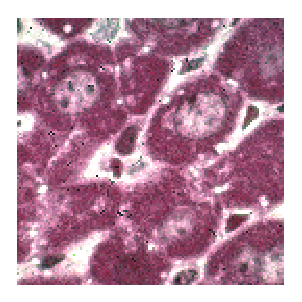
\epsfig{file = hepatocyte.eps, width = 1.6cm}}
 \subfigure[]{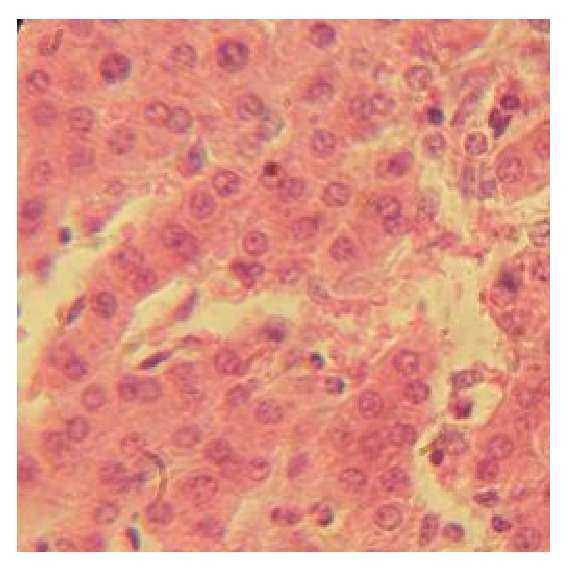
\epsfig{file = hepatique.eps, width = 1.6cm}}
 \subfigure[]{\epsfig{file = esrf.eps, width = 1.6cm}}
 \caption{\text{$128^2$} textured samples available to create volumetric data: (a) skeletal muscle sample artistically created;
          histology images of (b) striated cardiac muscle, (c) myocytes, 
	  (d-e) hepatocytes; (f) a slice from a SR$\mu$CT image of a trabecular bone sample.
          }
 \label{fig:sampleimages}
\end{figure*}

\section{\uppercase{Introduction}}
\label{sec:Introduction}

Realistic modeling of the human body is the current challenge in research of life sciences, projects around the world 
such as VPH-NOE (Virtual Physiological Human - Network of Excellence)\footnote{\url{http://www.vph-noe.eu/}} 
aim to create computer models for personalized and predictive health-care. 
The main goal is to create models capable of integrating
not only anatomical information but also physiological, mechanical and the biochemical processes related to the organ.

There are human anatomy models such as the Google Body Browser \footnote{\url{http://bodybrowser.googlelabs.com/body.html}}
or the Visible Body \footnote{\url{http://www.visiblebody.com/}},
they offer a detailed 3D view of the human body systems (digestive, nervous, skeletal etc.), and are based in {\bf surface representations}
of the structures. These models are organized in a multi-scale fashion, giving the possibility to navigate through 
the body system, they are mainly used as a learning tool, as they are not conceived to be used for 
patient-specific analysis or planning purposes.
These models have another limitation such as the lack of information at different scales \emph{e.g.} the structure of the bone tissue is not available.

Modeling different types of organs and tissues at the cellular level represents an interest for histology 
\emph{i.e.} the study of tissues. Histology plays an important role in the comprehension of 
morphological relationships between the organs and tissues, as it considers the structural organization 
or precise hierarchy of the organs with the smallest details. 
This represents an advantage as tissues are formed by cells, we could have structural information at different scales.

In this paper, we propose a method generic enough that is able to reproduce complex 3D objects, 
by using 2D textured samples.
Our method derives from Kopf's approach \cite{KFCODLW07}, it starts with a 2D reference image and 
by means of an energy optimization process described by Kwatra \cite{kwatra:2005:SIGGRAPH}, 
it is able to create a 3D texture that resembles the 2D image in every slice.
The reference 2D images can illustrate any textured element and can be of different kinds: i) artificial images artistically created for computer graphic design or medical atlases 
or ii) real images with very complex texture provided by digital microscopy of biomedical histological slices. 
Figure \ref{fig:sampleimages} show samples of textured images, available to produce different types of volumetric data.

%The texture synthesis optimization has the advantage of creating models, using one or multiple samples 
%to constraint the view in a different dimension, extra channels can be added to the exemplar, like distance maps 
%which are useful to code large texture features  \cite{Lefebvre:2006:ATS:1141911.1141921}. 
The texture synthesis optimization has the advantage to be able to constraint separately the axial, longitudinal and transversal planes of the 3D texture 
by taking into account one or multiple reference textures. 
Moreover, extra channels can be added to the exemplar, like distance maps when large texture features must be coded  \cite{Lefebvre:2006:ATS:1141911.1141921}. 

The method also maintains the global statistics of the sample by using a histogram matching 
approach presented by \cite{ROLLAND2000} and \cite{Heeger:1995:PTA:218380.218446}.
 
%This property gives the possibility to create images that are similar to those obtained by the image simulators.
%
In the remainder of this paper, we present in detail our method to synthesize realistic 3D textures modeling organic tissues and  
provide an overview of the different types of texture that can be generated. As we shall show in the section  \ref{sec:Evaluation}, 
the accuracy of the 3D synthetic texture is demonstrated by comparing statistical and morphological parameters computed from both the synthetic texture and the reference object. 
%
\section{\uppercase{Method}}
\label{sec:Methods}
\subsection{3D Texture Synthesis}
\label{sec:TextureSynthesis}

3D texture synthesis has been used before to create realistic solid objects,
giving the possibility to perform scattering simulations or cut through them.
Our approach is based on an energy proposed by \cite{kwatra:2005:SIGGRAPH} and defined by the following equation:
%The optimization is done similarly as

\begin{equation}
 E(o, \{e\} ) = \sum_{t} \sum_{i \in \{x, y, z\}} || o_{t, i} - e_{t, i} ||^r
 \label{equ:imagenergy} 
\end{equation}

It is based on a distance metric that compares the neighborhoods $x$, $y$, $z$ 
of a texel $t$ in the object $o$ and neighborhoods from the sample texture $e$. 
When minimized, using IRLS (iterative re-weighted least squares), 
the result is an increase of similarity between the sample and the synthetic object.

The procedure begins at a coarse resolution assigning random values from the sample to the synthetic object. 
Then, it alternates between a search phase where the closest neighborhoods are found 
and an optimization phase where the weighted average of every texel is calculated. 
When the optimization converges, it changes to a finer resolution level using linear interpolation.

\subsubsection{Search phase}
\label{sec:SearchPhase}

\begin{figure}[!h]
  \vspace{-0.2cm}
  \centering
  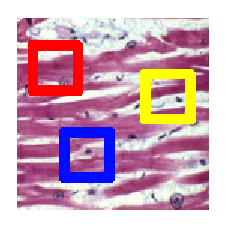
\epsfig{file = search_sample.eps, width = 2cm}
  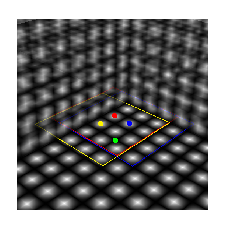
\epsfig{file = search_phase.eps, width = 4cm}
  \caption{9x9 red, blue and yellow neighborhoods for a slice in the volume, the center is represented by the colored dot.
           The green voxel is affected by multiple neighborhoods.}
  \label{fig:search_phase}
  \vspace{-0.1cm}
 \end{figure}

The sample image is divided into $9*9$ neighborhoods that overlap each other, these neighborhoods are vectorized \emph{i.e.} 
every texel from the neighborhood is stacked into a single vector. For RGB texels we have $9 * 9 * 3 = 243$ 
values in a single vector. It is possible to 
use a distance map as an extra channel by giving the algorithm a binary image as input, 
this is useful when the texture has large unstructured areas.
Once the vectors from the sample are constructed, we apply PCA 
(principal component analysis) \footnote{L. Smith 2002, A Tutorial on Principal Components Analysis; \url{www.cs.otago.ac.nz/cosc453/student_tutorials/principal_components.pdf}}
to reduce the dimensionality of each vector passing from $243$ to $18$ values approximately.

Reducing the vectors is a very convenient step, there are less values but we are still keeping $95\%$ of the relevant information.
The reduced vectors can be used to perform a standard closest neighborhood search in a high dimensional space. 
For this purpose, we use ANN library\footnote{ANN: A library for approximate nearest neighbor searching; \url{http://www.cs.umd.edu/~mount/ANN/} Mount, D. M. and Arya, S. 2006}.

\begin{equation}
 E(o, \{e\} ) = \sum_{t} \sum_{i \in \{x, y, z\}} \sum_{u \in N_i(t)} w_{t, i, u} ( o_{t, i, u} - e_{t, i, u} )^2
 \label{equ:imagenergy} 
\end{equation}
\begin{equation}
 w_{t,i} = || o_{t, i} - e_{t, i} ||^{r - 2}
 \label{equ:neighweight}
\end{equation}

During the search phase a weight for each neighborhood is calculated, for this purpose the energy function 
is written as equation \ref{equ:imagenergy} and the weight is calculated
as shown in equation \ref{equ:neighweight}. $N_i(t)$ represents the neighborhoods found in each dimension $x$, $y$, $z$ 
and $u$ is the texel in the neighborhood of $t$, this means that
a texel in the object is affected by multiple texels from different neighborhoods in the exemplar texture. 
The search is performed for every two texels $g_x = \{(i, 2 * j, 2 * k), \forall i, j, k \} $, $g_x$ 
is the voxel in a slice perpendicular to $x$. This is done similarly for $y$ and $z$, as shown in figure \ref{fig:search_phase}.
We set $r = 0.8$ to perform a robust optimization \cite{kwatra:2005:SIGGRAPH}.

Once the search phase is done the optimization phase takes place and it consists in averaging 
all the values found for each texel of the volume. 

\subsubsection{Optimization phase}
\label{sec:OptimizationPhase}

\begin{figure}
 \vspace{-0.2cm}
 \centering
 \subfigure[Exemplar textures.]{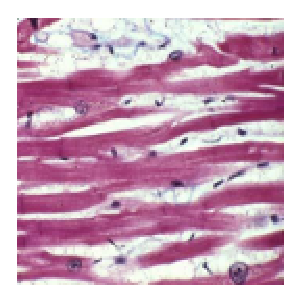
\epsfig{file = striescardiaques.eps, width = 1cm} 
            \hspace{1cm}
	    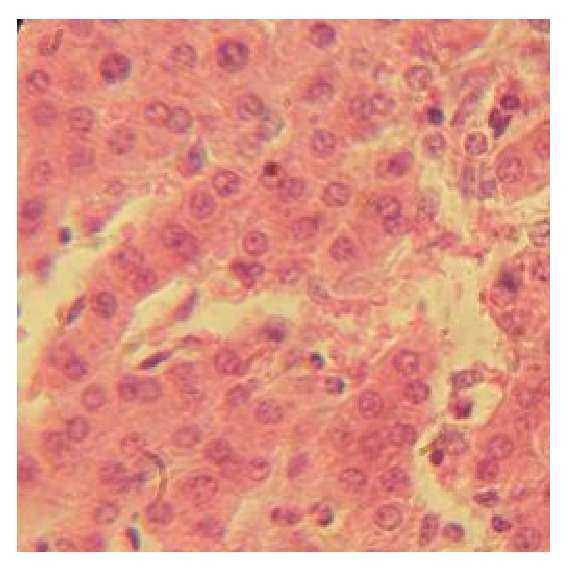
\epsfig{file = hepatique.eps, width = 1cm}}
 \subfigure[Generated volumes.]{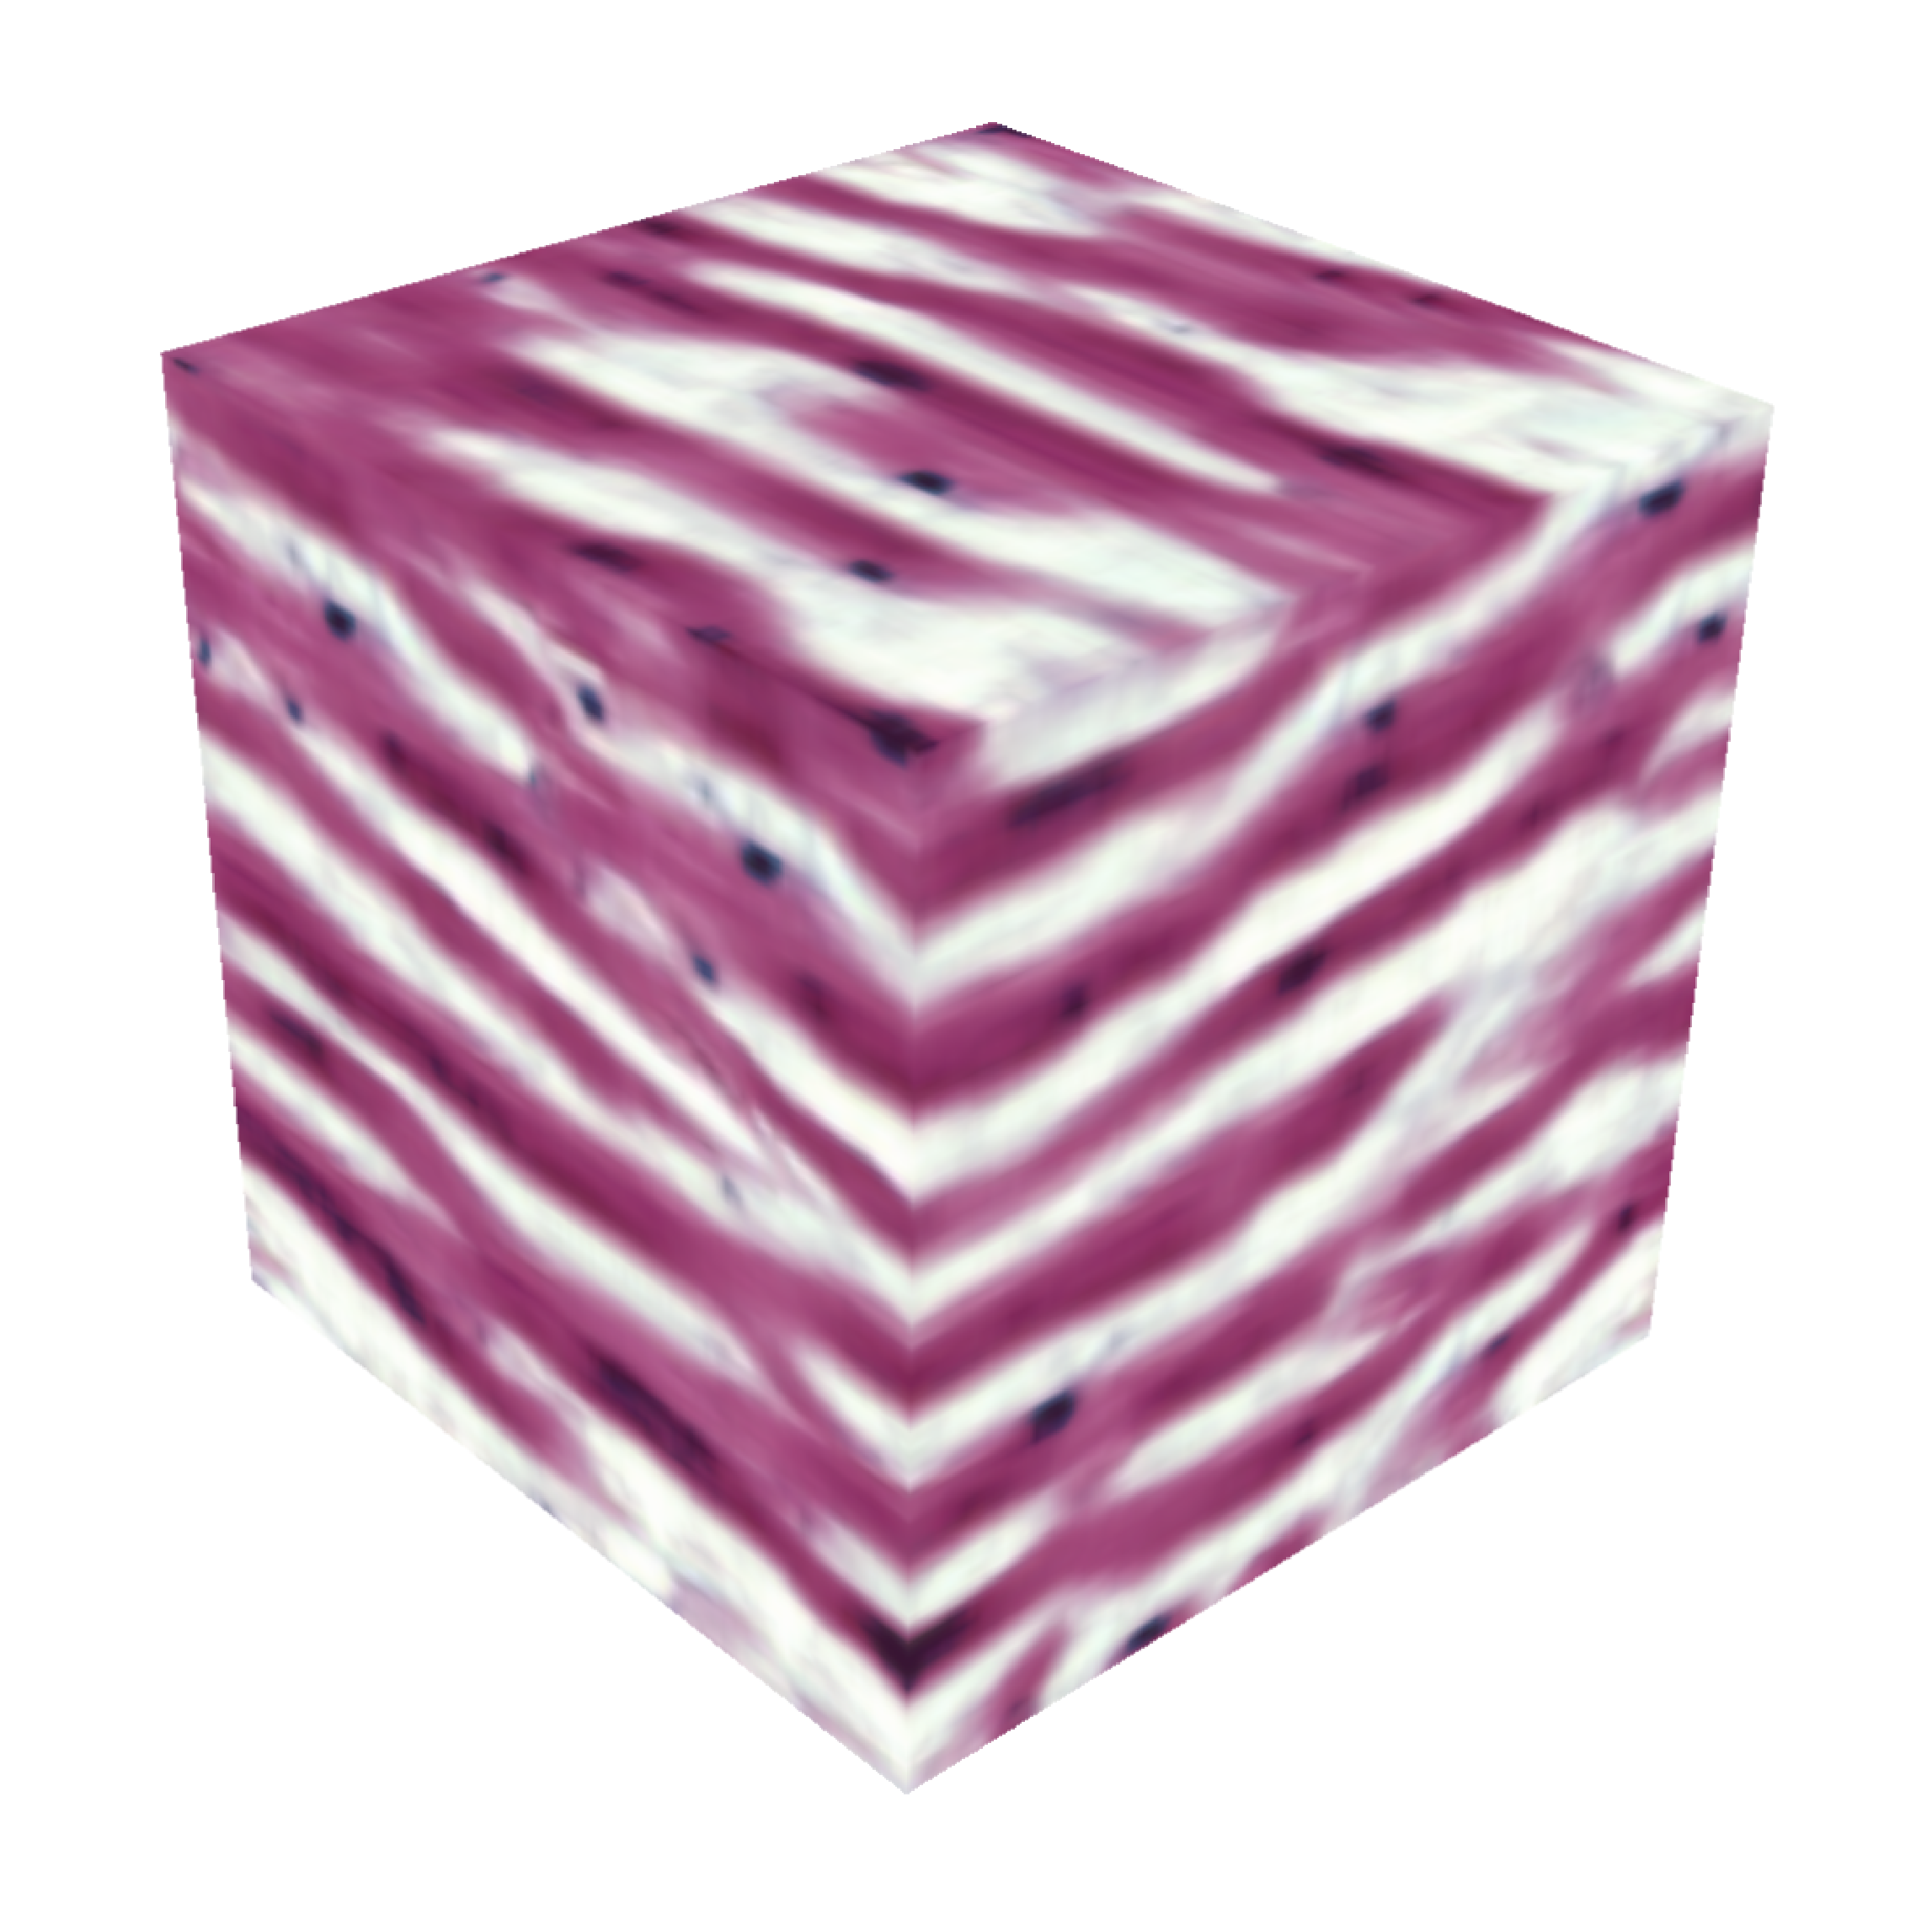
\epsfig{file = striescardiaquesVol.eps, width = 3cm}
			       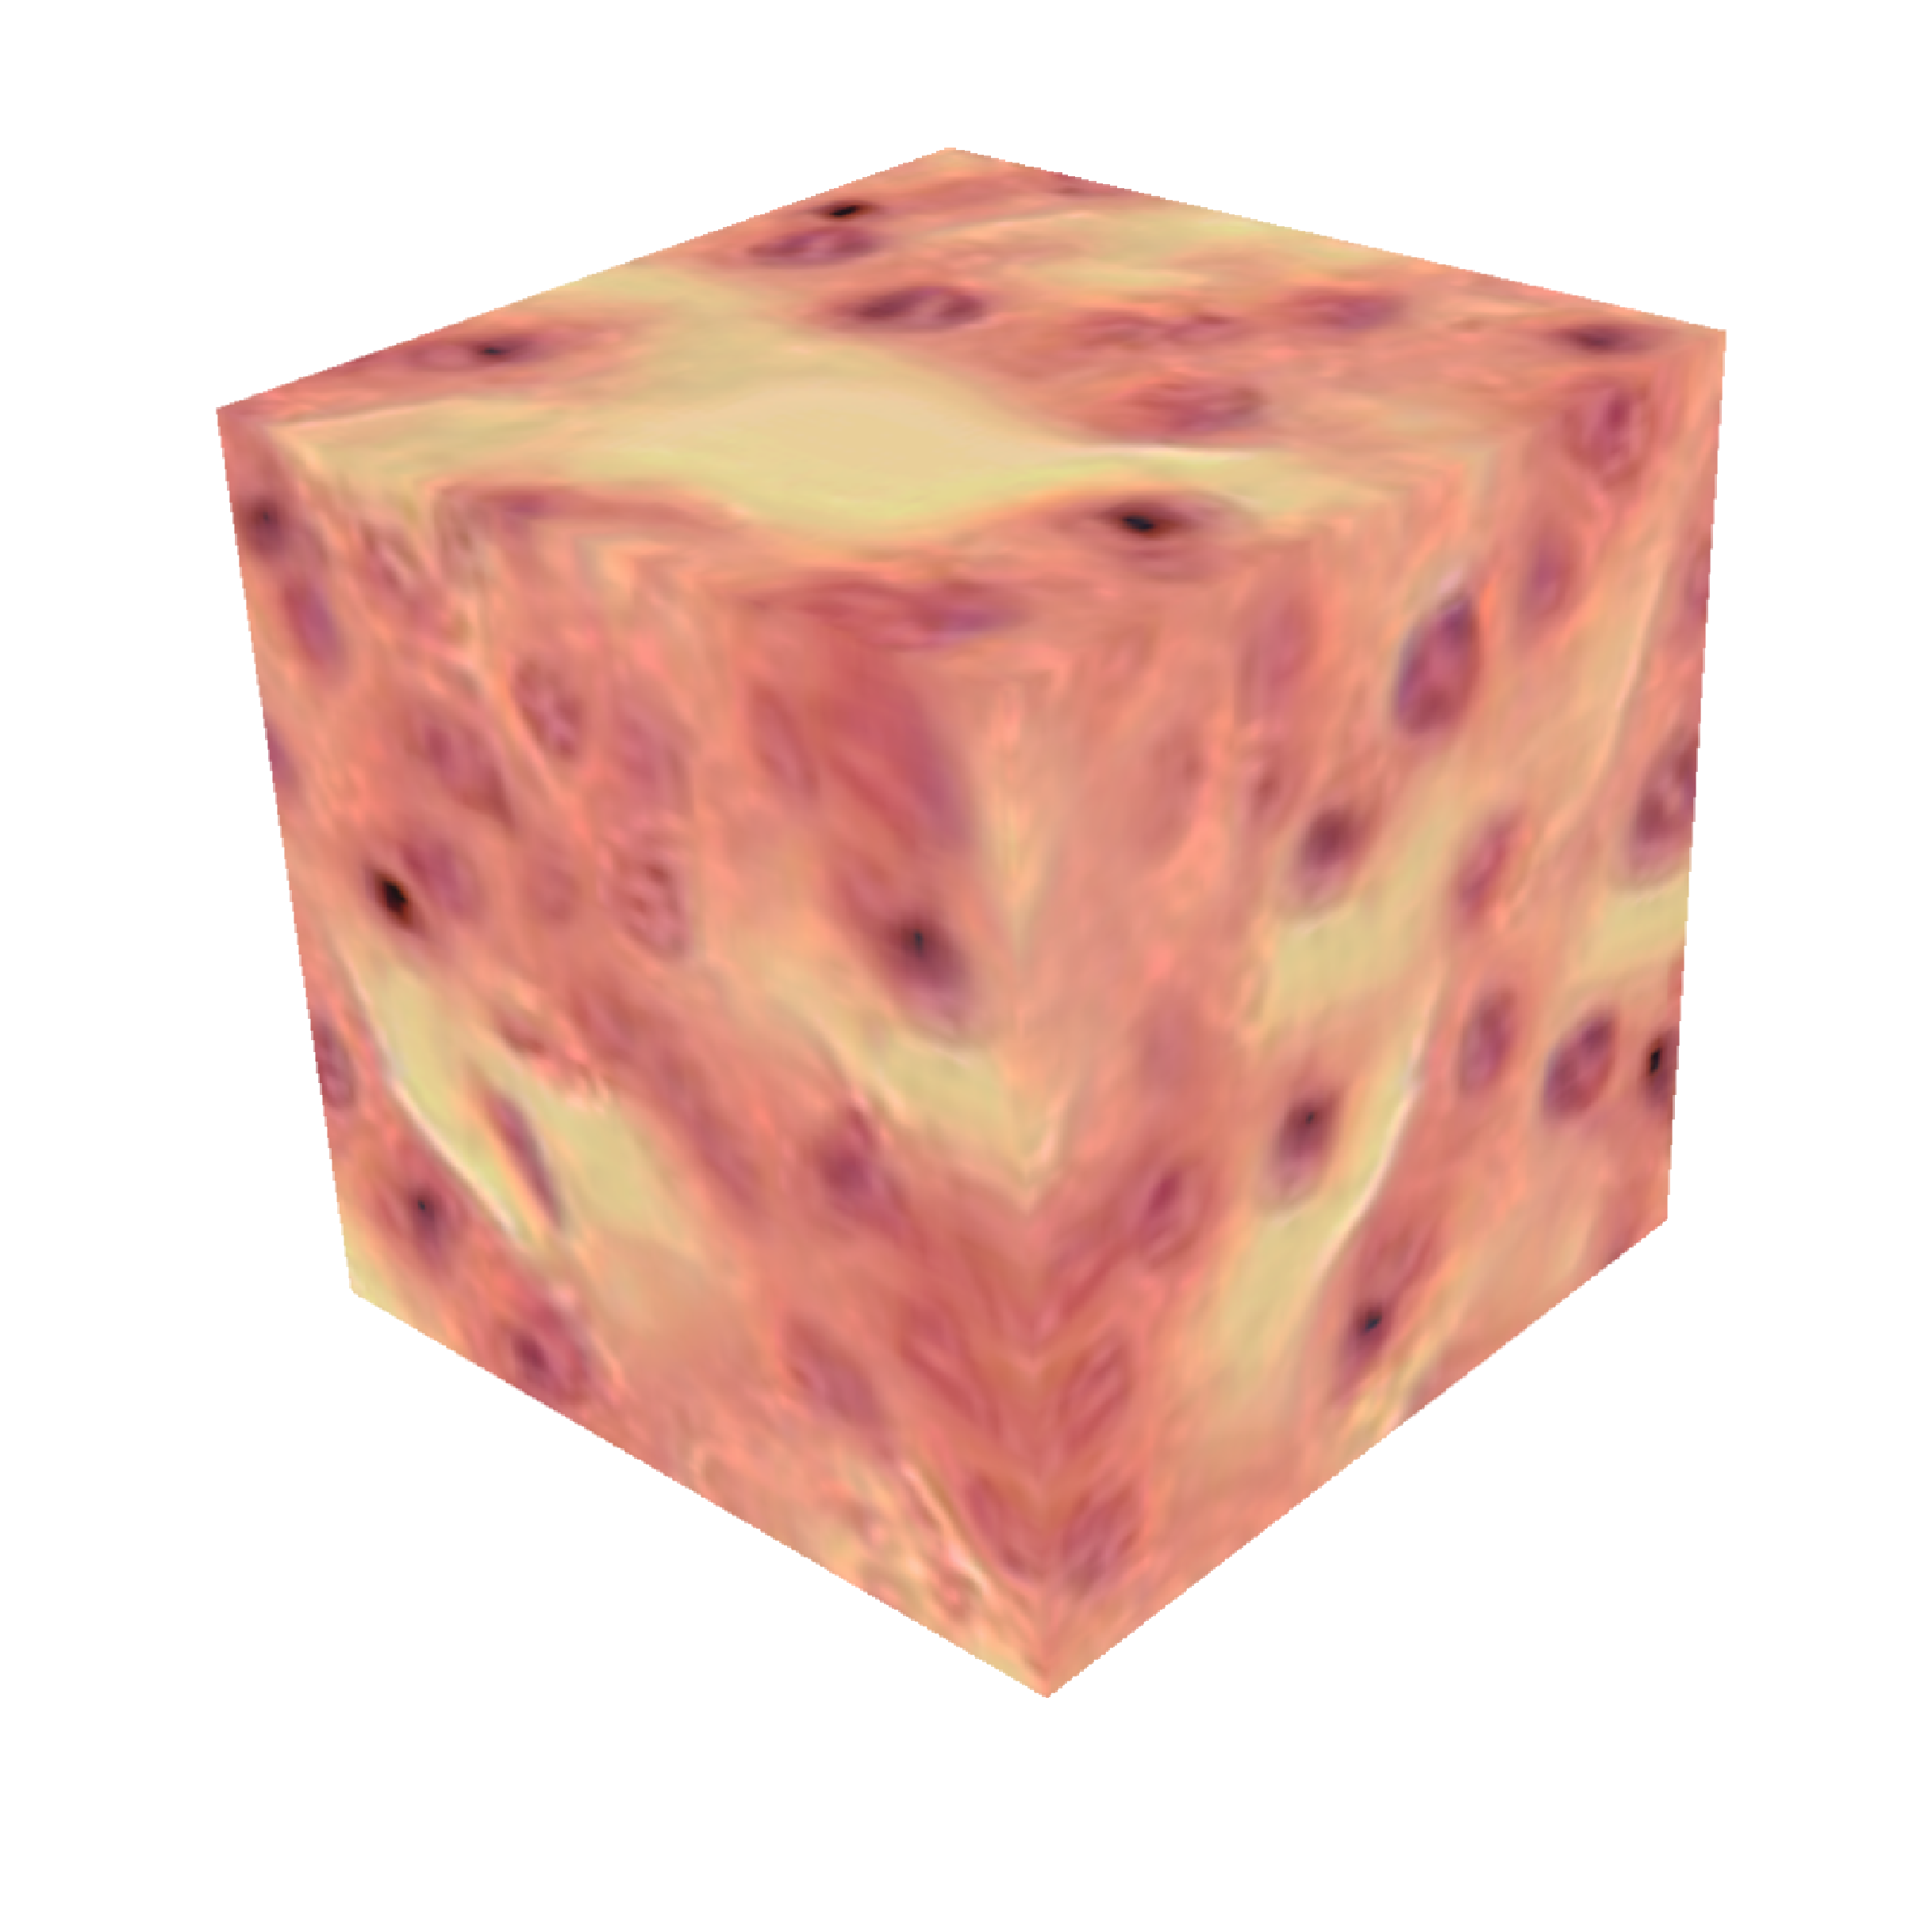
\epsfig{file = hepatiqueVol.eps, width = 3cm}
			      } 
 \caption{Results of isotropic synthesis. The striated cardiac muscle tissue (left)
          and liver cell tissue (right) were generated using a single reference texture 
          for the axial, longitudinal and transversal planes.
         }
 \label{fig:isotropicsynthesis}
 \vspace{-0.1cm}
\end{figure}

The optimization phase consists in averaging the values that affect one texel in the object. Note that
if the search phase is performed for every two texels as in \ref{sec:SearchPhase}, 
then the average will be for at most 75 texels (25 for each dimension).

\begin{equation}
 o_t = \frac{ \sum_{i \in \{x, y, z\}} \sum_{u \in N_i(t)} w_{u, i, t} * e_{u, i, t} }{ \sum_{i \in \{x, y, z\}} \sum_{u \in N_i(t)} w_{u, i, t} }
 \label{equ:texelaverage}
\end{equation}

Equation \ref{equ:texelaverage} shows the value of a texel in the object. 
When the texels present a high variability, the resulting object might be
blurred, in order to avoid this, 
clustering is performed to only average those texels that correspond to the principal cluster.

Following the optimization phase, the histogram matching is done to preserve the 
global statistics of the object relative to the exemplar. 

\subsubsection{Histogram Matching}
\label{sec:histogramMatching}

To perform histogram matching, the $CDF$ (cumulative distribution function) is calculated for both the exemplar 
and the object. 
Two $LUTs$ are constructed in order to perform faster calculations. 
The lookup table $LUT_o$ maps the RGB values of the object
to their corresponding value in the $CDF_o$, 
the lookup table $LUT_e$ maps the $CDF_e$
to the corresponding RGB values from the sample. 
The object is then modified by taking each of the texels $t$, using $LUT_o(t)$ to find the $CDF_o(t)$
and then using $LUT_e(CDF_o(t))$ to find the corresponding RGB value from the sample. The value of the object 
is then replaced by the corresponding value of the sample.

%\begin{figure}[!h]
%  \vspace{-0.2cm}
%  \centering
%   {\epsfig{file = histogramCDFLUT.eps, width = 5.5cm}}
%  \caption{CDF of the exemplar and the object with the corresponding $LUT$ functions.}
%  \label{fig:search_phase}
% \vspace{-0.1cm}
% \end{figure}

\section{\uppercase{Results}}
\label{sec:Results}

\begin{figure}
 \vspace{-0.2cm}
 \centering 
 \subfigure[Exemplar textures.]{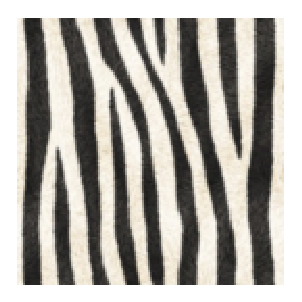
\epsfig{file = zebra.eps, width = 1cm}
            \hspace{1cm}
	    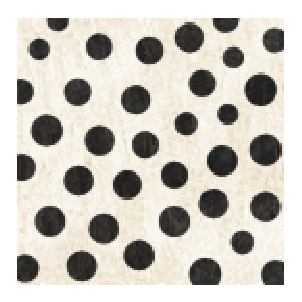
\epsfig{file = zebraAx.eps, width = 1cm}
	   }\\
 \subfigure[Generated volume.]{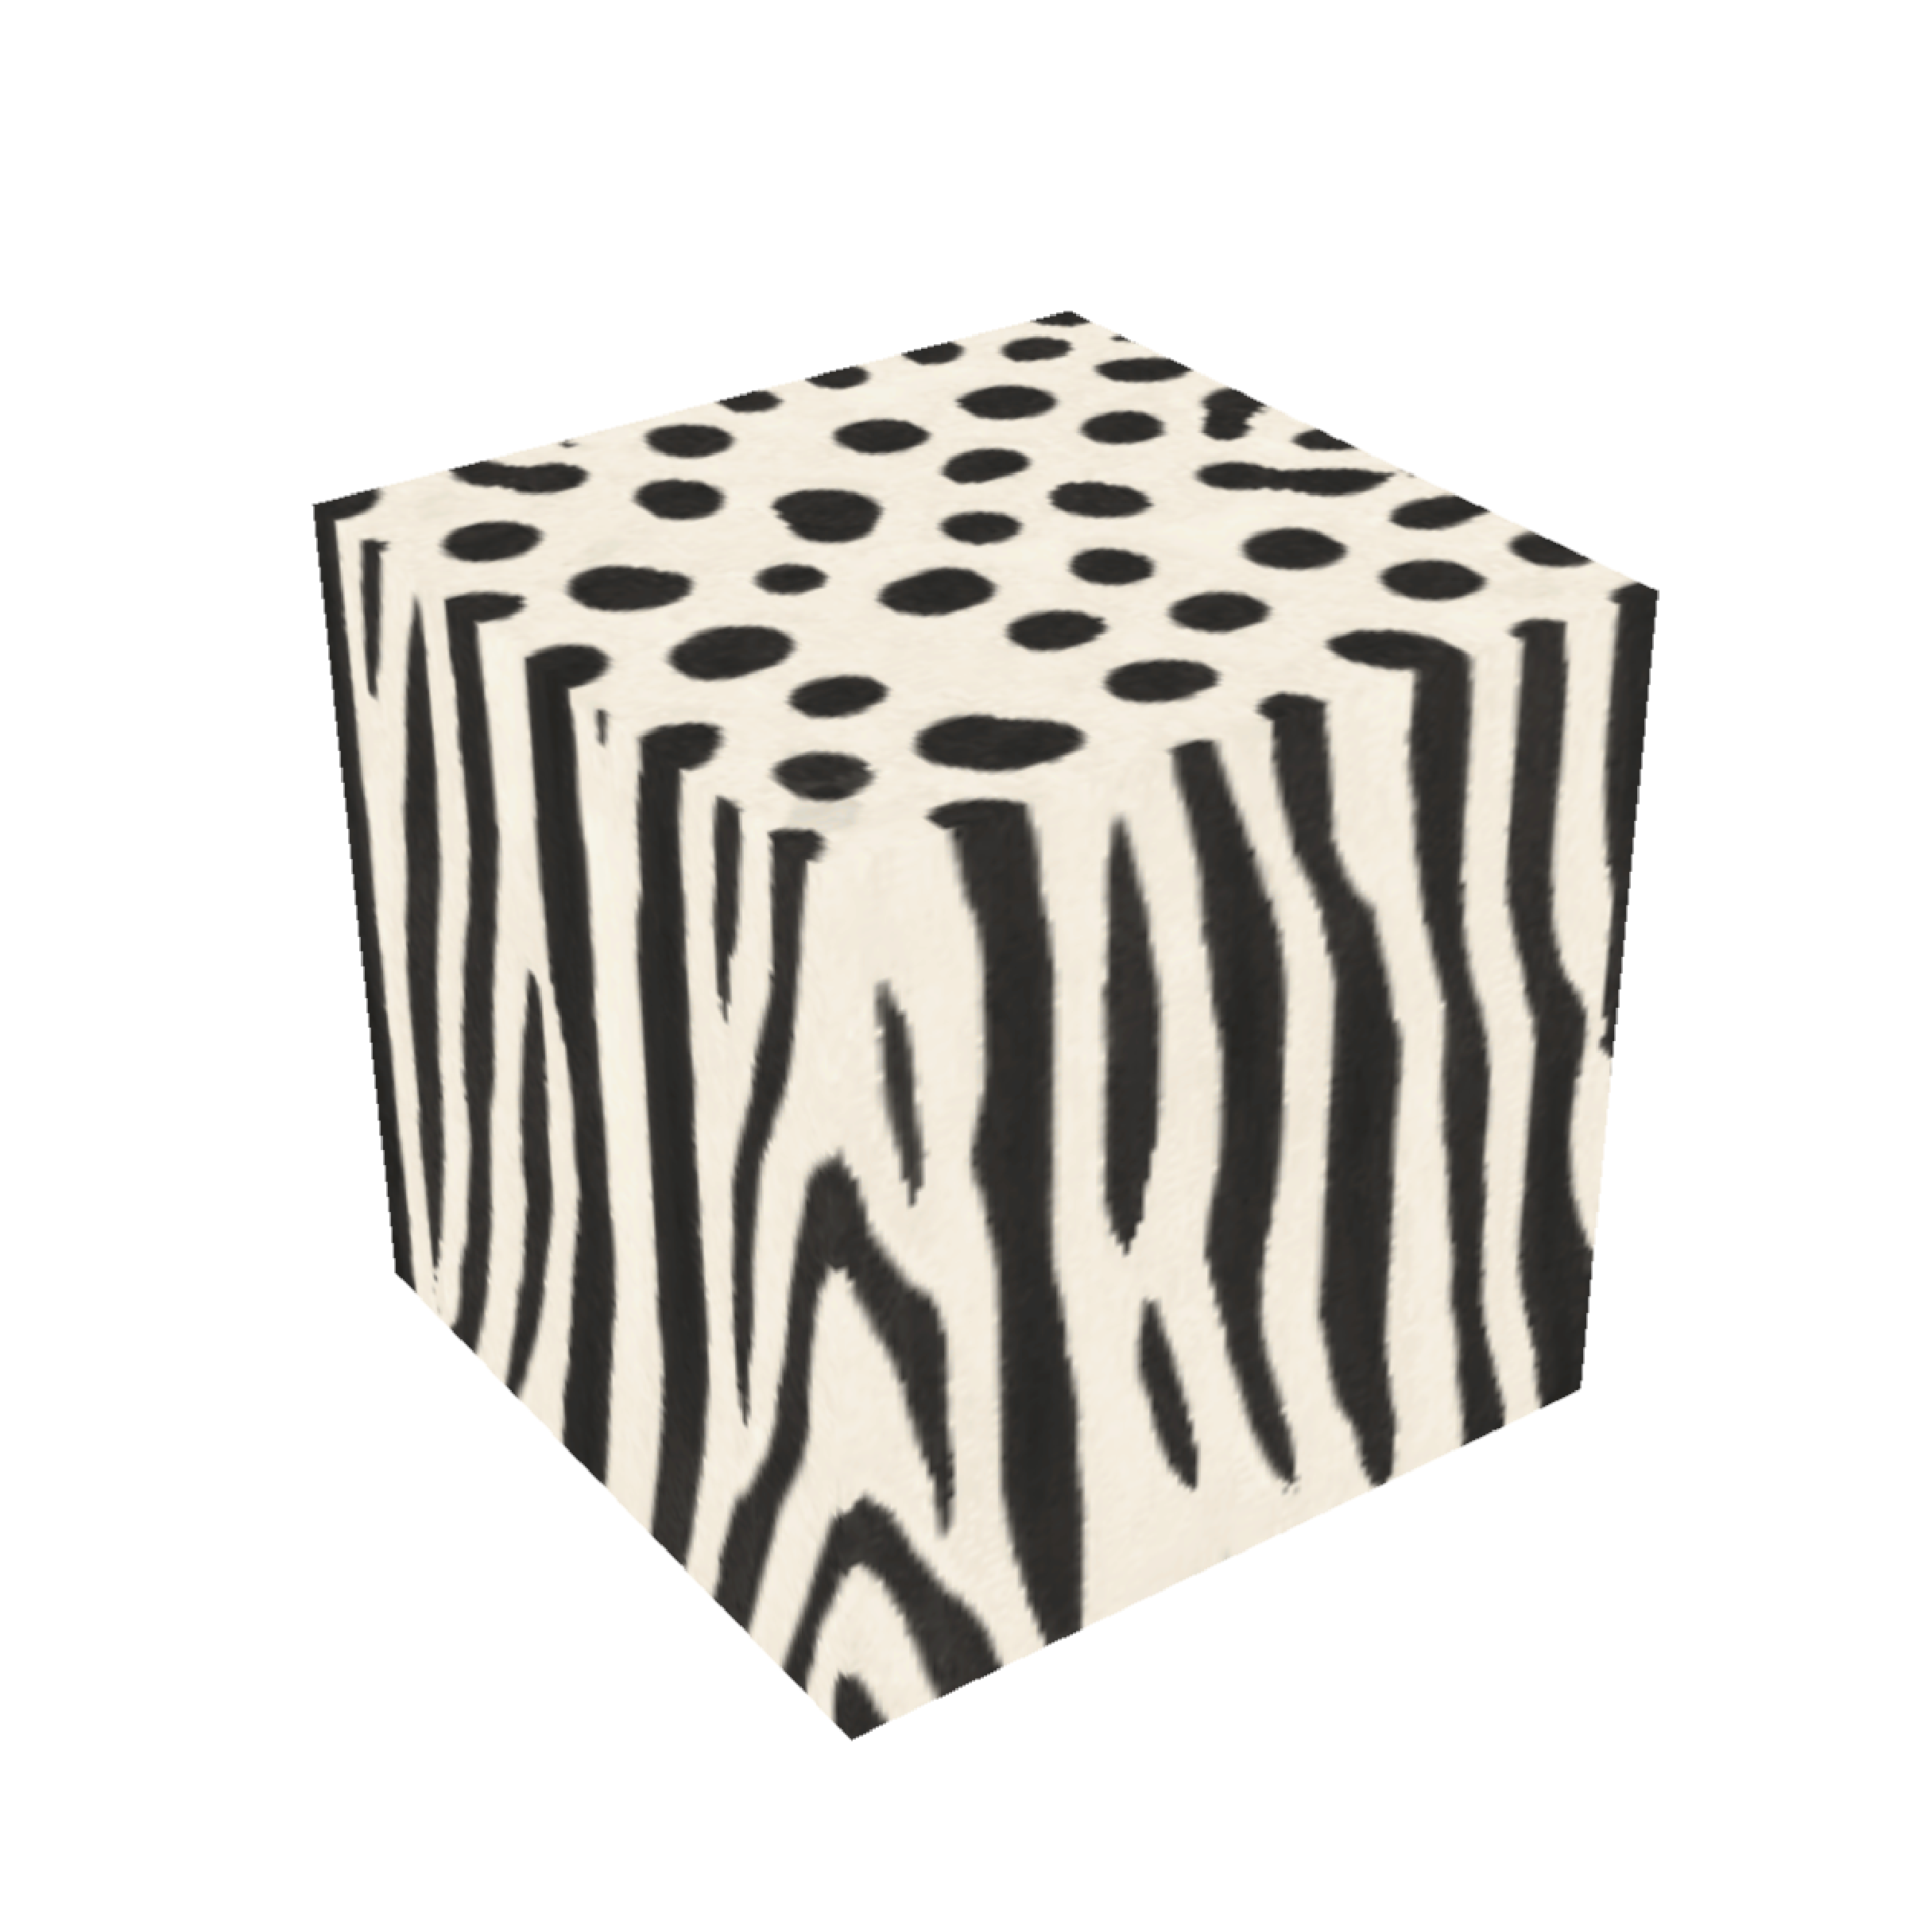
\epsfig{file = zebraVol.eps, width = 3cm}}
 \subfigure[Surface rendering.]{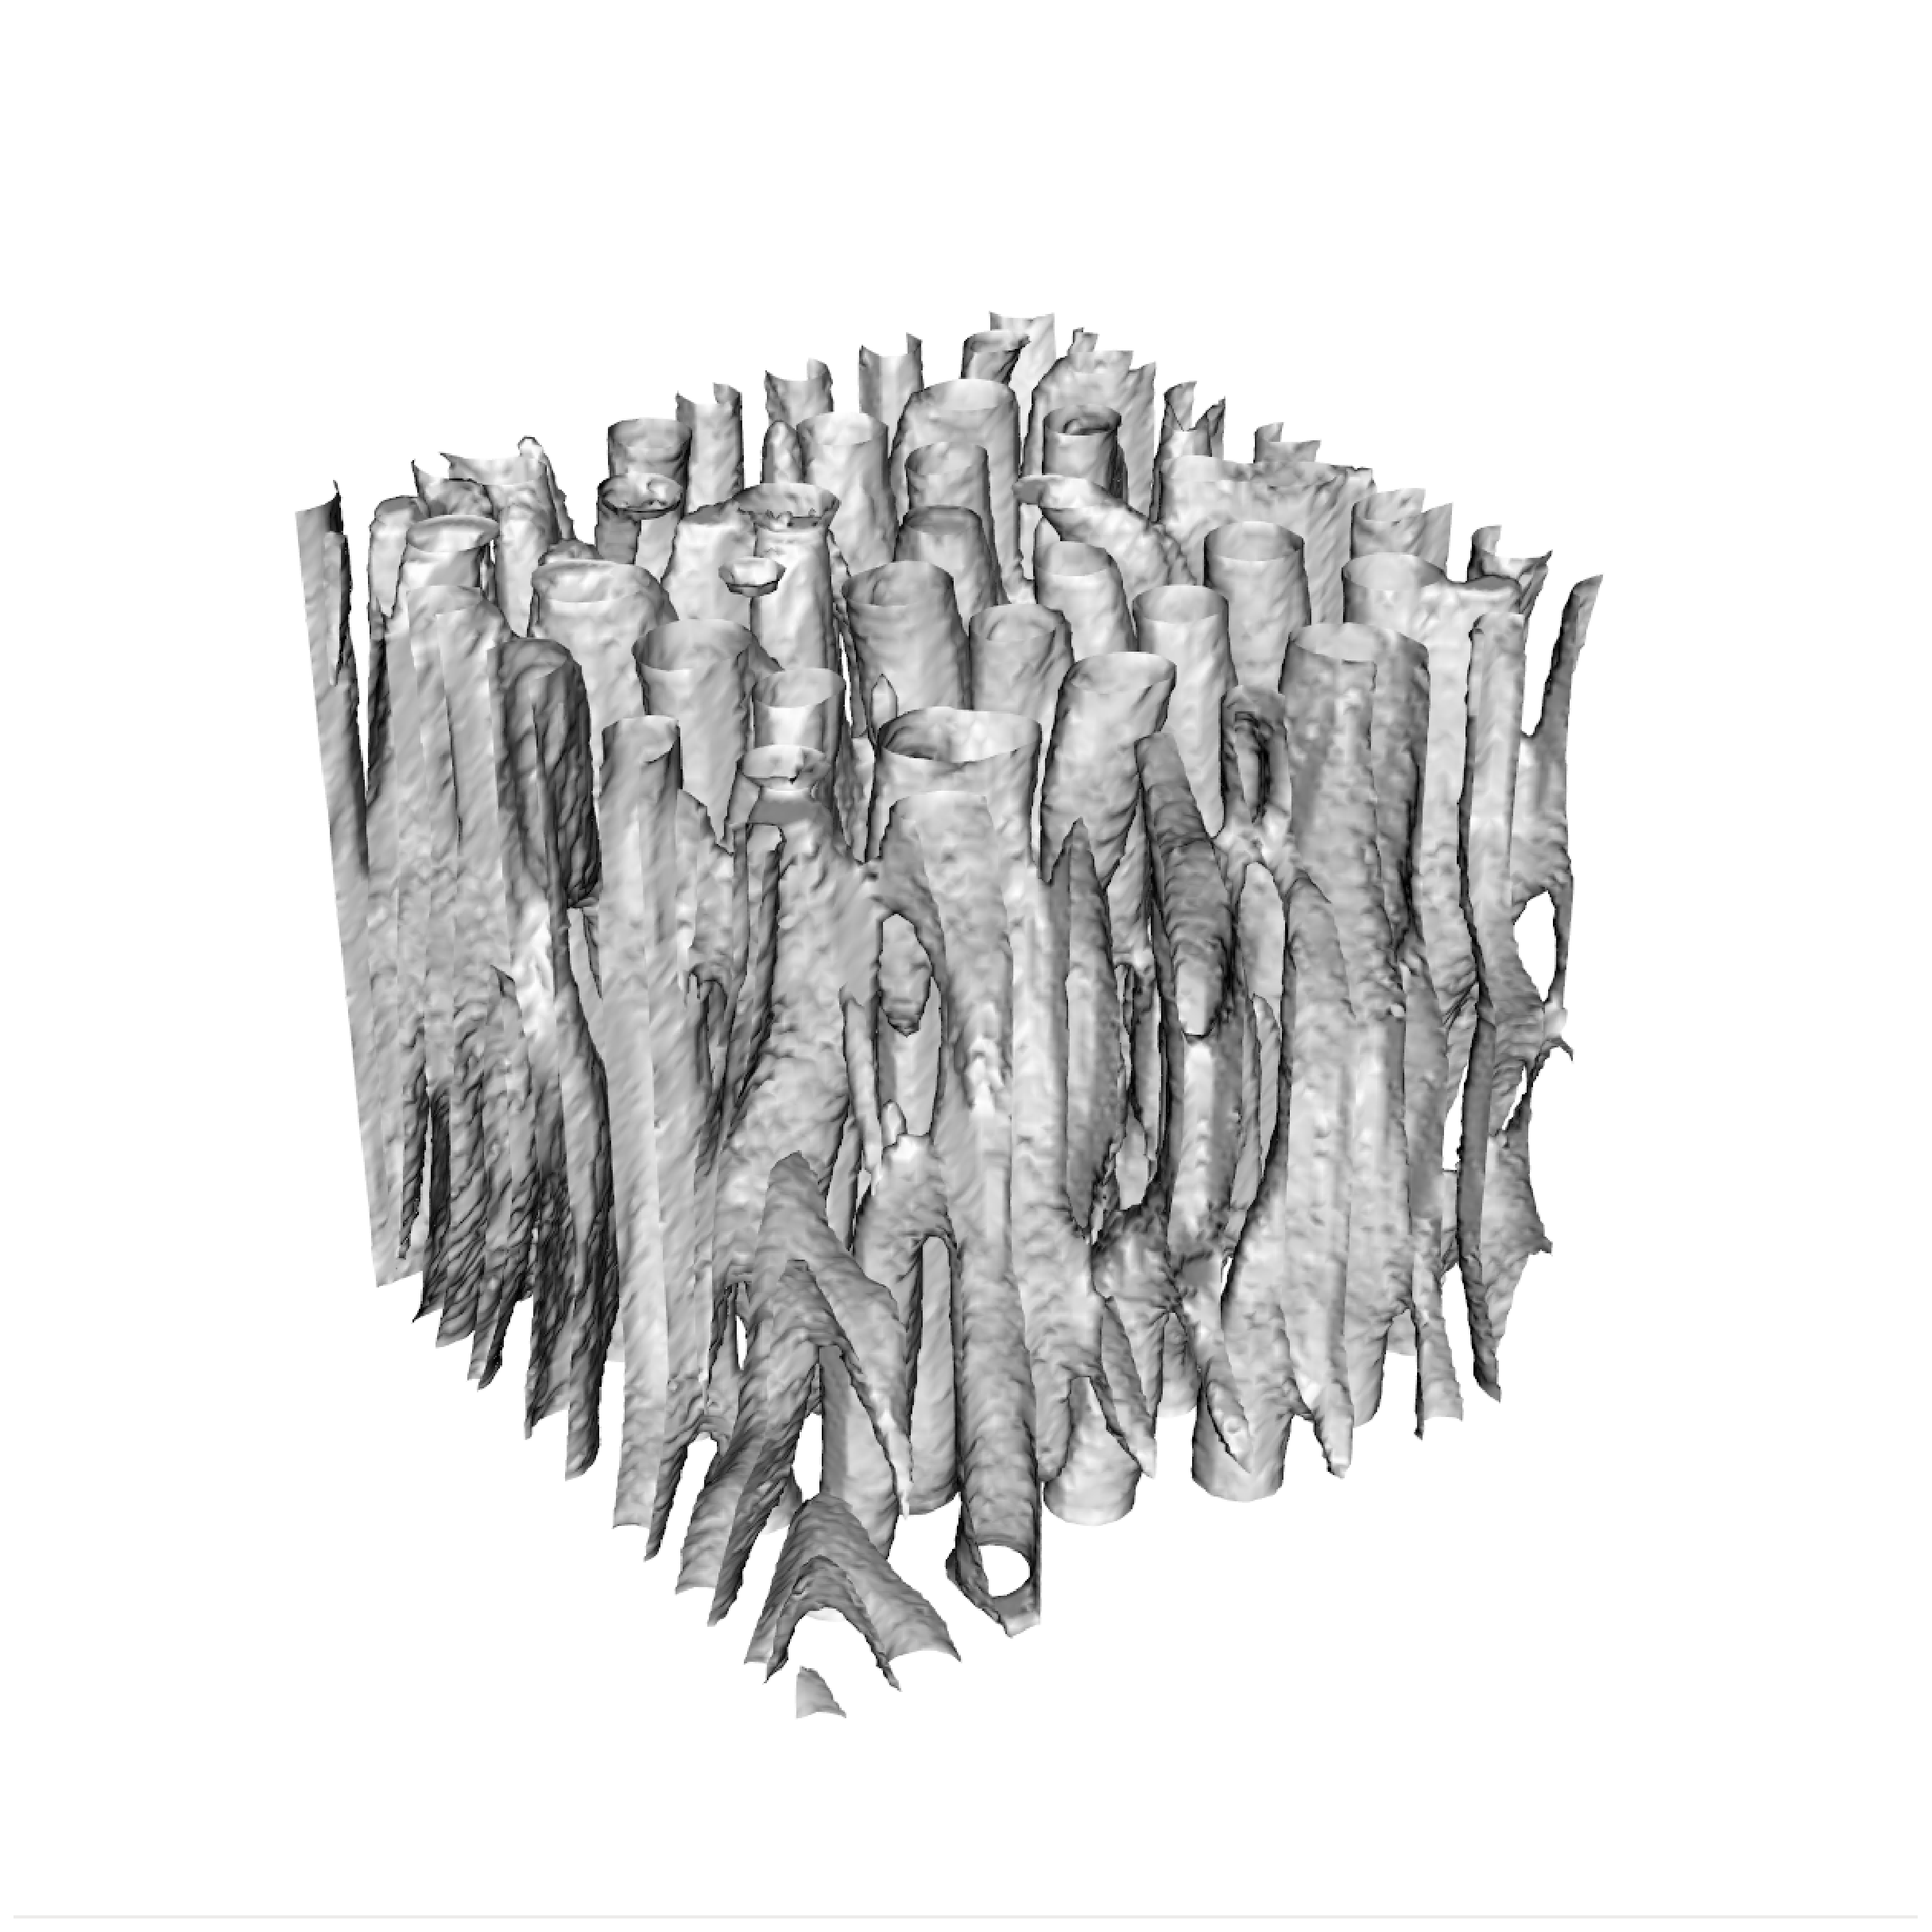
\epsfig{file = zebraSurf.eps, width = 3cm}}				  
 \caption{Results of anisotropic synthesis. The optimization was performed using the zebra texture to constraint the longitudinal and transversal planes. The dot texture was used in the axial plane.}
 \label{fig:3DAnisotropicTexture}
 \vspace{-0.1cm}
\end{figure}

The algorithm was implemented in C++ using ITK\footnote{\url{http://www.itk.org}} for image processing and 
VTK\footnote{\url{http://www.vtk.org}} for visualization. 
Using ITK allowed the image processing to be performed in parallel, thus gaining computational time.
Synthetic 3D images of both $128^3$ pixels and $256^3$ pixels were generated using different type of textures, from histology images 
acquired with a digital microscope.% and image samples from IRM image acquisitions. 

\subsection{Isotropic texture from a 2D exemplar texture}

Figure \ref{fig:isotropicsynthesis} shows some results when the same exemplar is used
to perform the optimization in the perpendicular planes of each three axis. Our method allows the 3D synthesis of the striated 
cardiac muscle tissue and the liver cell tissue from only one histology slice. 
It can be noted that any axial, longitudinal or transversal slice of the volume is similar to the reference texture without being, however, identical.

\subsection{Anisotropic texture from many 2D exemplar textures}

Figure \ref{fig:3DAnisotropicTexture} shows the result of selecting two different textures 
to constraint the optimization.
Selecting the zebra texture for the longitidunal and transversal planes with the dot pattern for the axial plane generated cylinder like structures. 
When rendering the surface of the object, we can see that the generated structure 
is very complex and consists of tubes that join and separate at arbitrary slices.
This synthetic structure was used in our lab to test Brownian simulation algorithms 
that reveal the environment's structures.

\subsection{Anisotropic texture constrained by additional masks }

\begin{figure}
 \centering 
 \subfigure[Exemplar textures + binary masks.]{
\epsfig{file = myocyte.eps, width = 1cm}
	    
\epsfig{file = myocyteSgMask.eps, width = 1cm} \hspace{1cm}
	    
\epsfig{file = myocyteAx.eps, width = 1cm}
	    
\epsfig{file = myocyteAxMask.eps, width = 1cm}
	   } \\
 \subfigure[Longitudinal view of the volume.]{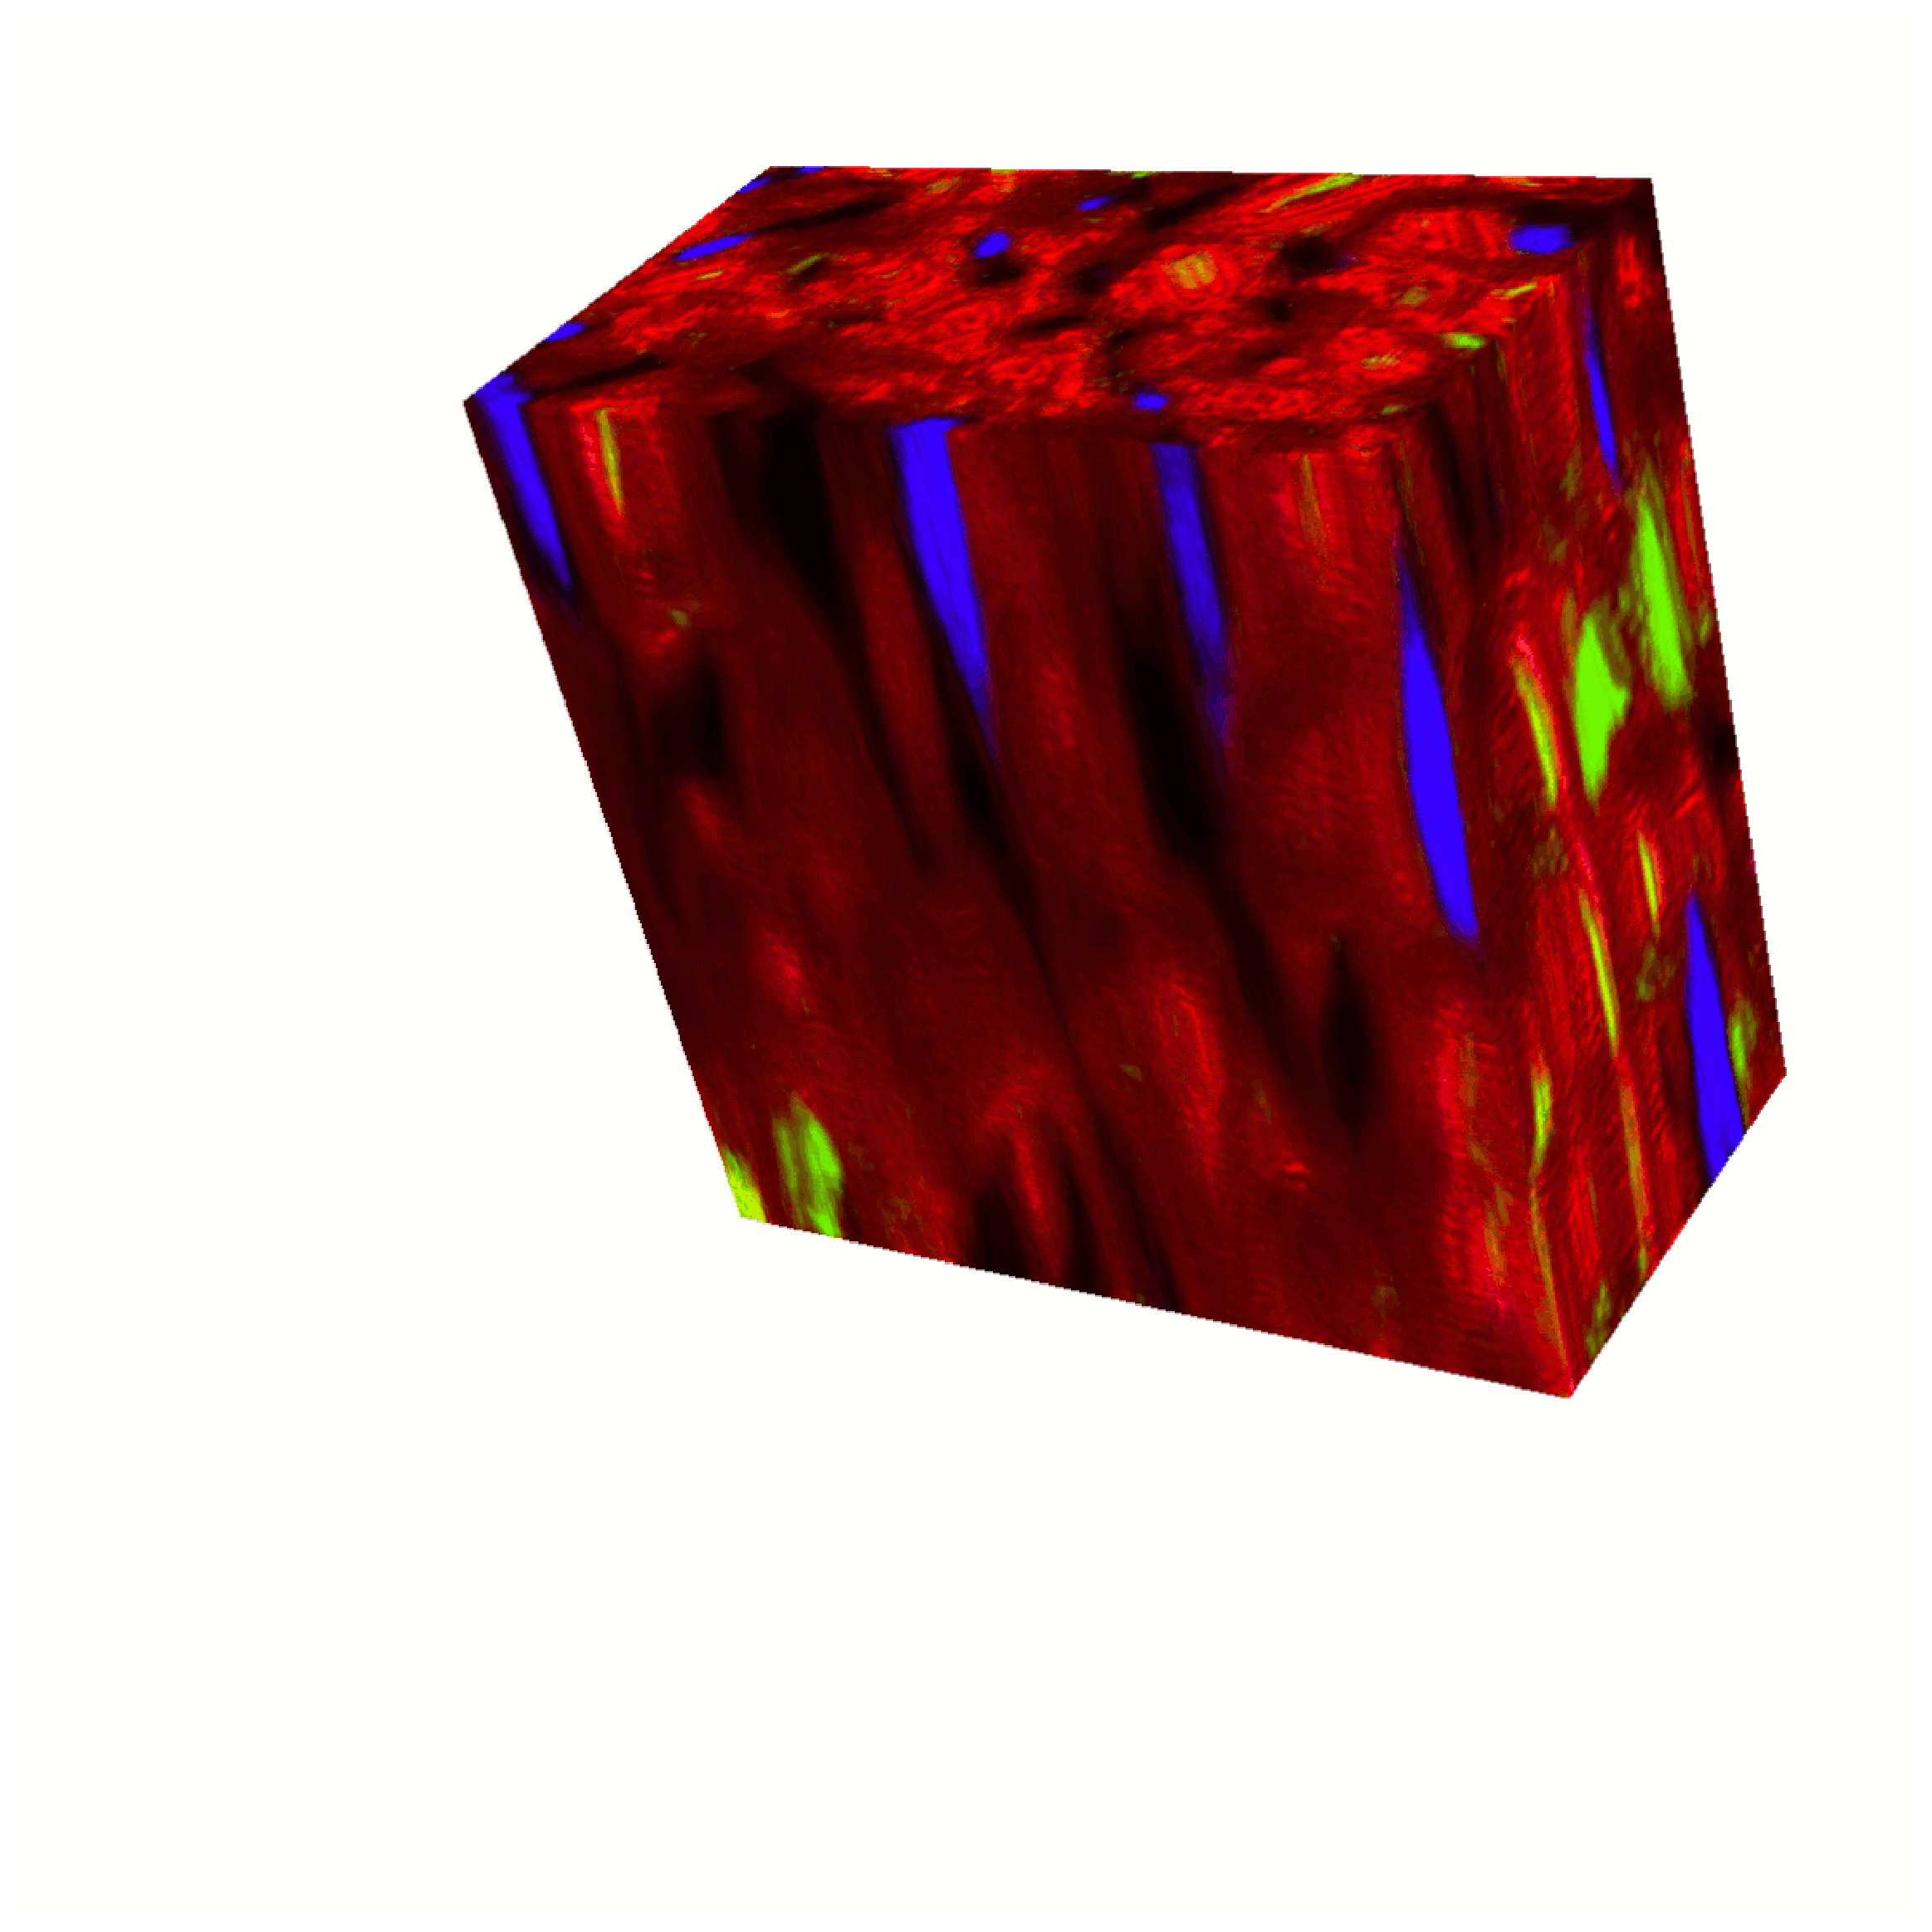
\epsfig{file = myocyteSgVol.eps, width = 3cm}}
 \subfigure[Axial view of the volume]{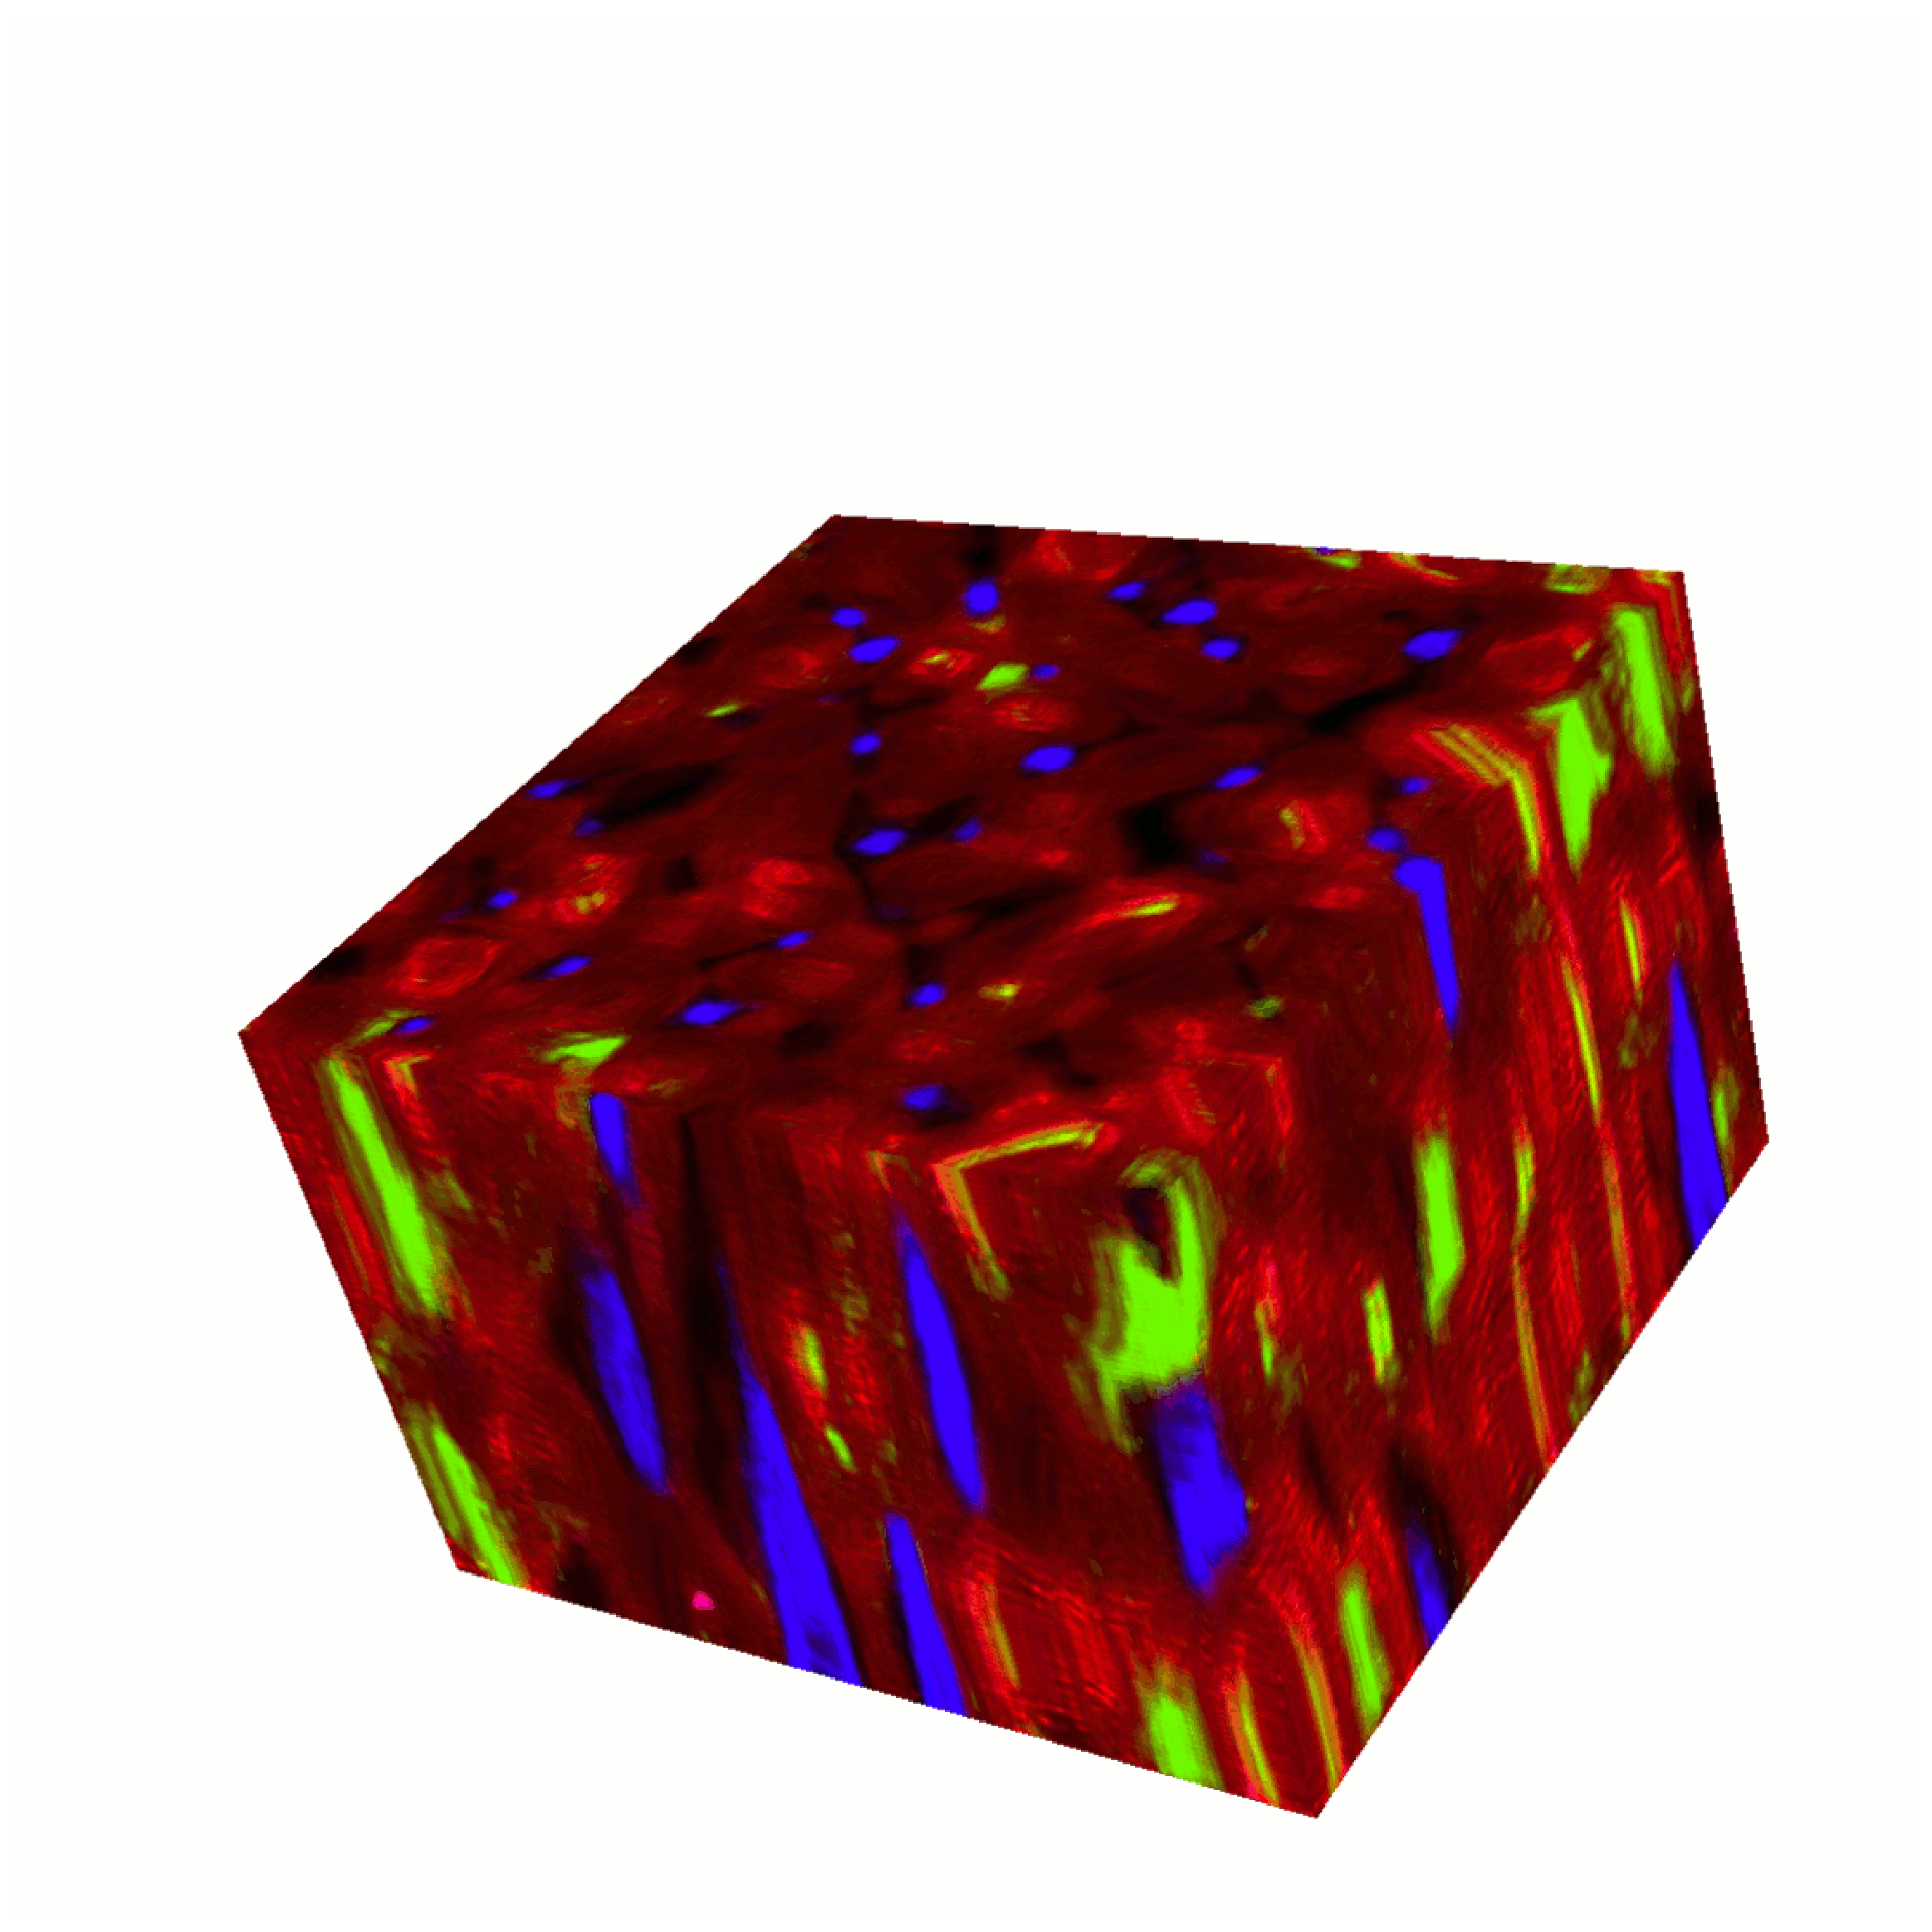
\epsfig{file = myocyteAxVol.eps, width = 3cm}
				  }
 \caption{Results of anisotropic synthesis starting from two different textures and their additional binary masks.}
 \label{fig:3DAnisotropicTextureAndMask}
\end{figure}

Figure \ref{fig:3DAnisotropicTextureAndMask} shows the synthesis results using different exemplar textures obtained from confocal images\footnote{\url{http://www1.ic.ac.uk/medicine/people/p.camelliti/}} and extra channels provided by signed Euclidean distance maps computed from  binary masks. 
The 3D texture representing a myocyte cell tissue are quite representative of cells organisation (myocytes in red and fibroblasts in blue).The anisotropy of the cells is conspicuous and the contrast of staining is well preserved thanks to the use of the binary masks. 
%The 3D texture represents a myocyte cell tissue.


One main advantage of our method is to generate a 3D tissue from 2D information. 
Up to now, it was impossible for the biologist or the physician to have a 3D representation 
of the cell tissue, since it is technically very difficult or even impossible to have 
an axial resolution as good as those in the slice. 
Thanks to our approach, the experts can get a virtual 3D representation of the tissues 
that are close to reality without being it.

\section{\uppercase{Evaluation and Discussion}}
\label{sec:Evaluation}

We propose to assess the quality of our synthetic 3D texture according to two criteria: 
statistical and morphological accuracy. 
As the ultimate goal of our work is to produce a 3D texture as close as possible to the reference object, 
we will compare statistical and morphological features computed from the reference object with to those 
computed from the synthetic texture. 

\subsection{\uppercase{Statistical assessment }}
\label{sec:Statistics}

\begin{table}[h]
\centering
\begin{tabular}{|c|c|c|c|}
  \hline
  & & Mean & St. Dev  \\
  \hline
  \multirow{2}{*}{Red} & $e$ & 189.6  & 34.7  \\
		       & $o$ & 188.7 & 34.0 \\
  \hline
  \multirow{2}{*}{Green} & $e$ & 142.4 & 70.2 \\
		         & $o$ & 141.4 & 69.3 \\
  \hline
  \multirow{2}{*}{Blue} & $e$ & 168.8  & 48.7 \\
		        & $o$ & 168.0  & 48.1 \\
  \hline
\end{tabular}
\caption{Means and standard deviations for the RGB channels of the exemplar and the object}
\label{tab:statshisto} 
\end{table}

Figure \ref{fig:histograms} shows the histograms from the exemplar texture and the synthesized object shown 
in figure \ref{fig:isotropicsynthesis}. The total number of pixels in the texture are $128^2 = 16384$ and
$128^3 = 2097152$ for the volume. Note that when a randomly chosen slice is taken from the volume, 
the global statistics are still preserved. 
Table \ref{tab:statshisto} contains the means and the standard deviations calculated from the histograms, the values
from the object are similar to those of the exemplar with a variation lower than 1$\%$ for the means and lower than 2$\%$ for the standard deviations. 

\begin{figure}
 \vspace{-0.2cm}
 \centering  
 \subfigure[Exemplar]{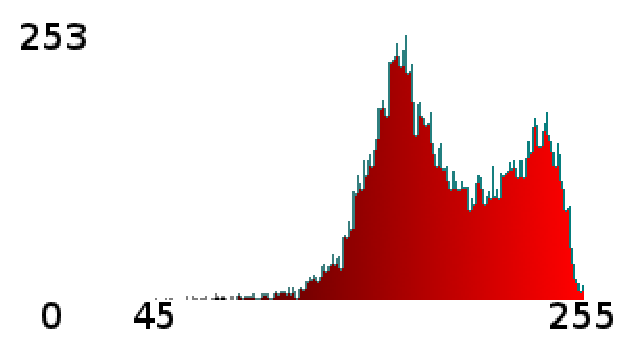
\epsfig{file = redHistoSample.eps, width = 2.5cm} 
	    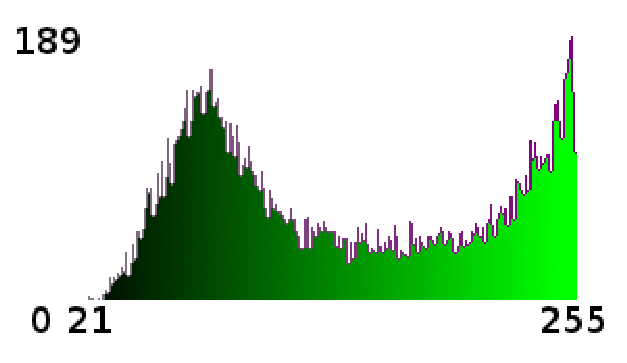
\epsfig{file = greenHistoSample.eps, width = 2.5cm}
	    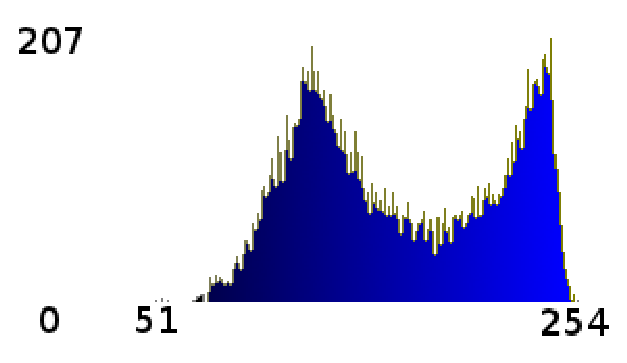
\epsfig{file = blueHistoSample.eps, width = 2.5cm}
           }\\
 \subfigure[Object]{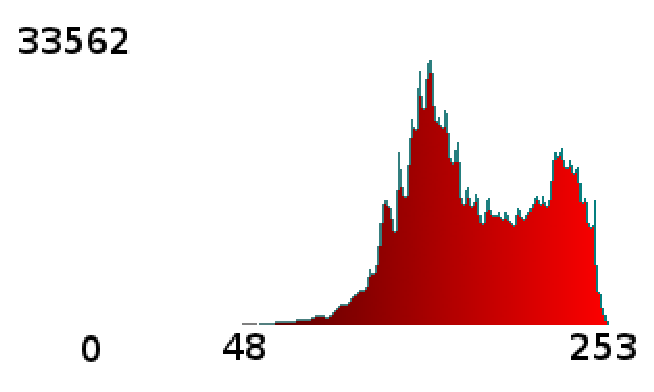
\epsfig{file = redHistoObject.eps, width = 2.5cm}
	    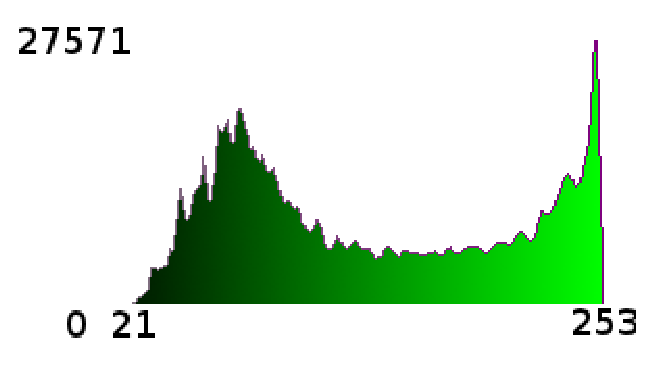
\epsfig{file = greenHistoObject.eps, width = 2.5cm}
	    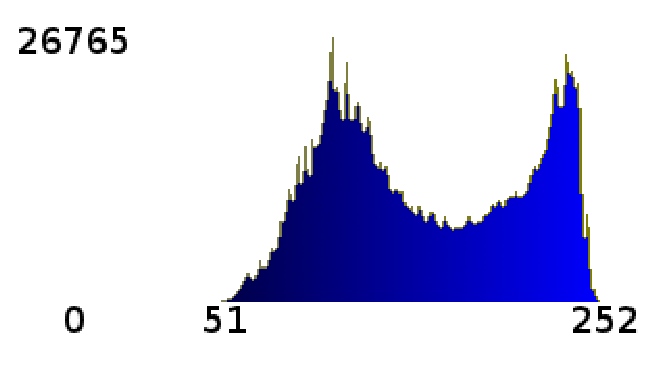
\epsfig{file = blueHistoObject.eps, width = 2.5cm}
           }
 \caption{RGB histograms of the exemplar and the object for the striated
          cardiac muscle shown in figure \ref{fig:isotropicsynthesis}.}
 \label{fig:histograms}
 \vspace{-0.1cm}
\end{figure}

\subsection{\uppercase{Morphological assessment}}
\label{sec:Morphology}

We propose to quantitatively assess the accuracy of the morphological structure given by our 
synthetic 3D texture. For this study, we generate a 3D texture from images provided 
by Synchrotron Radiation Computed Micro-Tomography (SR$\mu$CT). 
These images were acquired few years ago on beam-line ID19 at the European Synchrotron Radiation Facility 
(ESRF) in Grenoble for the needs of a study focused on osteoporosis. 
Osteoporosis is a bone fragility disease leading to spontaneous bone fractures and 
characterized by a bone mass reduction and a bone structure deterioration. 
3D Synchrotron Radiation Computed Micro-Tomography (SR$\mu$CT) provided 3D high resolution 
images with an isotropic voxel of 10 $\mu$m width and a volume size of 
$330 * 330 * 330$ pixels helpful to assess trabecular bone architecture \cite{revol2002}. 
Therefore, we have at our disposal a set of twelve 3D SR$\mu$CT images obtained from 
twelve calcaneus bone samples excavated from deceased human. 
For the test of our method, we worked on decimated SR$\mu$CT images with a resolution of 
80$\mu$m and a size of $83 * 83 * 83$ voxels. 
At this resolution, the signal to noise ratio is still high enough to extract trabecular 
bone from the background by simple automated thresholding. 
This binarizing step is needed for the computation of the bone parameters.

\begin{figure}
 \vspace{-0.2cm}
 \centering  
 \subfigure{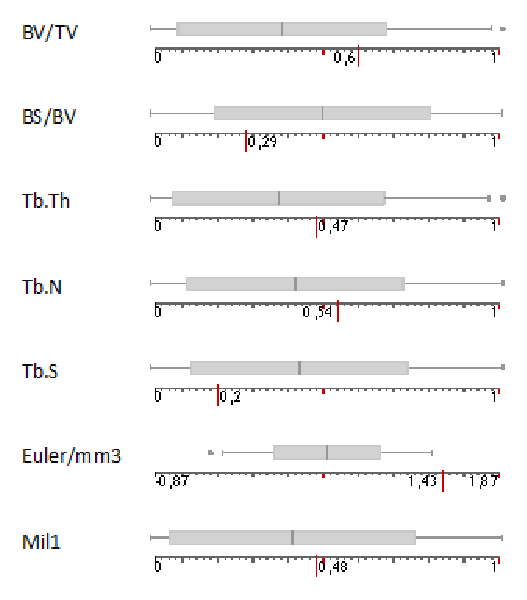
\epsfig{file = esrfEvaluation.eps, width = 5.5cm}}
 \caption{Box plots for morphologic and topological architecture of bones.}
 \label{fig:bone_parametres}
 \vspace{-0.1cm}
\end{figure}

We computed morphologic and topological architecture parameters similar to those used in histomorphometry 
but computed on three-dimensional images from the set of the twelve volumes. 
A 3D MIL (Mean Intercept Length) method based on a three-dimensional version of the directed 
secant algorithm was chosen to produce many parameters related to the trabecular 
bone morphology \cite{Hipp97} and the Euler number was computed to estimate the bone topology. 
We considered the seven following parameters: Partial Bone Volume (BV/TV), Bone Surface to 
Bone Volume ratio (BS/BV), Trabecular Thickness (Tb. Th), Trabecular Number (Tb. N), 
Trabecular Separation (Tb. Sp) and Mean Intercept Length (MIL1). The connectivity was estimated by the Euler number 
(Euler/mm3) implemented following the method described in 
\cite{Odgaard93} and normalized by the total volume. 
The higher the Euler number's value, the less connected the bone structure is.

We generated by our method a 3D SR$\mu$CT-like texture ($128 * 128 * 128$ voxels) from two random 
reference slices ($83 * 83$ pixels) taken into one out of the twelve SR$\mu$CT volumes.  
We binarized the texture in order to extract the virtual bone architecture by the same automated 
thresholding than that used for the set of SR$\mu$CT volumes. 
Then we assess the accuracy of the virtual bone structure by comparing the bone parameters computed 
from the set of SR$\mu$CT images with those computed from the synthetic 3D volume.

Figure \ref{fig:bone_parametres} displays the box plots associated to each bone parameter obtained 
from the set of SR$\mu$CT images. As our aim is not focused on the analysis or 
the interpretation of these parameters but only on the comparison of them, 
we normalized each parameter by the range between their maximum and minimum values. 
The score of the synthetic texture is displayed on the scale line under each box plot by a 
long red line. It can be noticed that for all the morphologic parameters the score for the 
virtual bone is spread in a range lower than +/- one standard deviation from the mean 
value obtained from the SR$\mu$CT set, thus proving its resemblance with the architecture of real bone. 
For the topology parameter (Euler/mm3), the score is slightly higher than the maximum value 
obtained with the SR$\mu$CT set, but that remains satisfying. It means that the virtual bone 
structure has a somewhat lower connectivity than the reference set. It could represent a high degree of osteoporosis.  

\begin{figure}
 \vspace{-0.2cm}
 \centering
 \subfigure[Exemplars + binary masks]{\epsfig{file = esrf.eps, width = 1cm}  
	    \epsfig{file = esrfMask.eps, width = 1cm} \hspace{1cm}
	    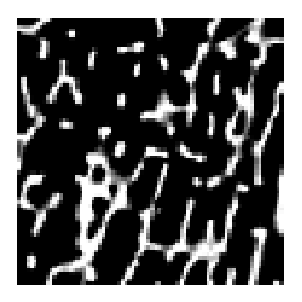
\epsfig{file = esrf1.eps, width = 1cm}
	    \epsfig{file = esrf1Mask.eps, width = 1cm}
	   }
\subfigure[Generated volume.]{
			      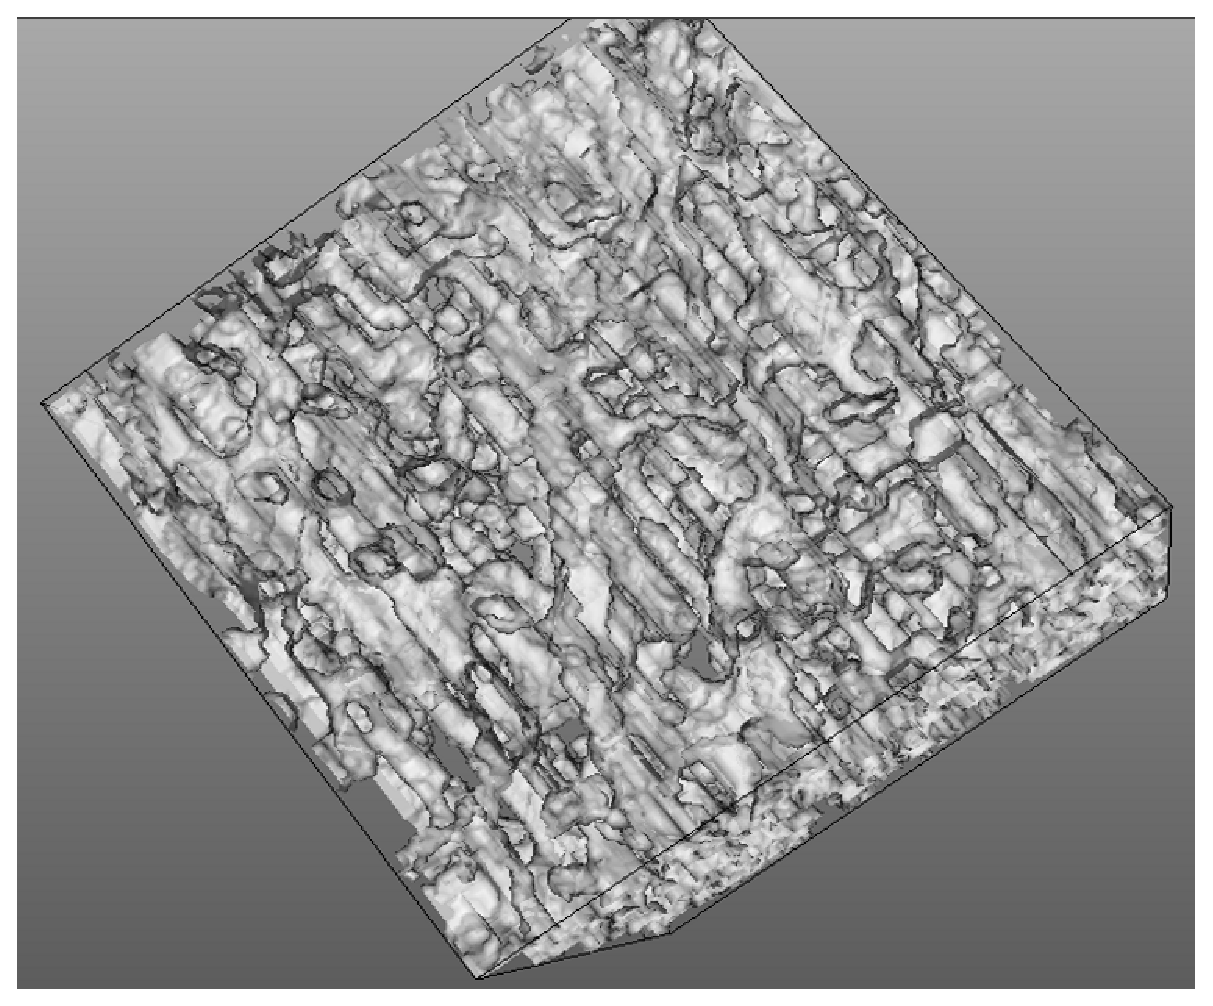
\epsfig{file = texture3D-SRCTSynthetic.eps, width = 3cm}
			    }
\subfigure[Real volume.]{
			      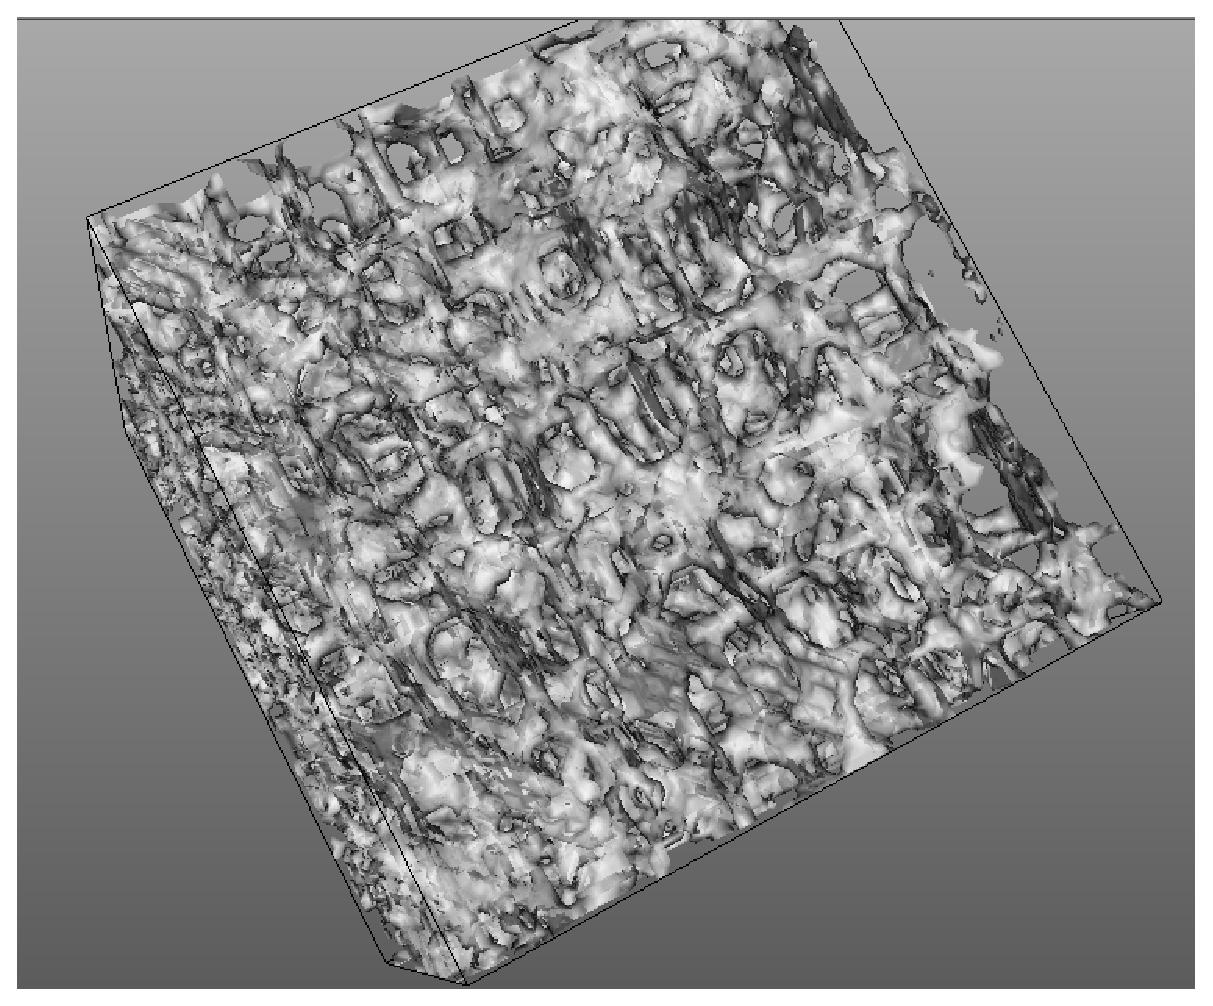
\epsfig{file = texture3D-SRCT.eps, width = 3cm}
			     }
 \caption{Anisotropic synthesis with additional binary masks. Surface rendering of trabecular bone architecture obtained with the synthetic texture and the SR$\mu$CT image.}
 \label{fig:bone_surface_rendering}
 \vspace{-0.1cm}
\end{figure}

In Figure \ref{fig:bone_surface_rendering}, the surface of the virtual bone is 
compared to the surface of the 3D SR$\mu$CT image from which were taken 
the reference slices for the texture synthesis. 
We retrieve visually the similarity demonstrated by the bone parameters.

\section{\uppercase{Conclusion}}
\label{sec:Conclusions}

Our method allows to create realistic organic tissue from small samples acquired by a digital microscope or
other image acquisition devices such as Synchrotron Radiation Computed Micro-Tomography. We demonstrated quantitatively the accuracy of 
the synthetic texture from both statistical and morphological points of view. 
Latter tests showed that our synthetic objects like the zebra-dot 3D texture can be useful for simulation especially in the framework of Brownian simulation. 
In future work, we will use our method to enhance surface models. We will aim at coupling texture synthesis with minimal skeleton 
representations such as the m-reps developed by Pizer \emph{et. al} \cite{Pizer:2003:DMM:945881.945883}
and reproducing the interior of the organs at multi-scale levels using 2D samples of tissue. 


\vfill
\bibliographystyle{apalike}
{\small
\bibliography{3D_Texture_Synthesis_for_Modeling_Realistic_Organic_Tissues}}

\vfill
\end{document}